\documentclass[a4paper, twoside, english, 12pt]{book}

\usepackage{graphicx,subfig,acronym,fancyhdr,listings,longtable,verbatim,enumerate,courier,caption,tabularx,pdfpages}
\usepackage[latin1]{inputenc}
\usepackage[hyphens]{url}
\usepackage[pdftex,colorlinks]{hyperref}
\usepackage[top=3.0cm, bottom=2.5cm, left=2.5cm, right=2.5cm, bindingoffset=1cm, includefoot]{geometry}

\setcounter{secnumdepth}{3}

\hypersetup{
		bookmarksnumbered,
		linkcolor=black, 		% Color for normal internal links.
		anchorcolor=black,		% Color for anchor text.
		citecolor=black,		% Color for bibliographical citations in text.
		filecolor=magenta, 		% Color for URLs which open local files.
		menucolor=red, 			% Color for Acrobat menu items.
		pagecolor=red, 			% Color for links to other pages
		urlcolor=blue, 			% Color for linked URLs.
}

\urlstyle{rm}

\setlength{\parindent}{0pt} 
\setlength{\parskip}{2ex}
\addtolength{\headheight}{0.5pt}
\addtolength{\footskip}{0.5pt}


\usepackage{fancyhdr}
\pagestyle{fancy}
\fancyhead{}
\fancyhead[RO]{\bfseries\rightmark}
\fancyhead[LE]{\bfseries\leftmark}
\renewcommand{\headrulewidth}{0.5pt}
\cfoot{\thepage} 


\begin{document}

\definecolor{darkgray}{rgb}{0.95,0.95,0.95}
\lstset{ %
language=c,                % choose the language of the code
basicstyle=\small,       % the size of the fonts that are used for the code
numbers=left,                   % where to put the line-numbers
numberstyle=\footnotesize,      % the size of the fonts that are used for the line-numbers
stepnumber=0,                   % the step between two line-numbers. If it is 1 each line will be numbered
numbersep=5pt,                  % how far the line-numbers are from the code
backgroundcolor=\color{darkgray},  % choose the background color. You must add \usepackage{color}
showspaces=false,               % show spaces adding particular underscores
showstringspaces=false,         % underline spaces within strings
showtabs=false,                 % show tabs within strings adding particular underscores
frame=single,   		% adds a frame around the code
tabsize=2,  		% sets default tabsize to 2 spaces
captionpos=b,   		% sets the caption-position to bottom
breaklines=true,    	% sets automatic line breaking
breakatwhitespace=false,    % sets if automatic breaks should only happen at whitespace
escapeinside={\%*}{*)}          % if you want to add a comment within your code
}

\pagenumbering{roman}
\pagestyle{fancy}


% Latex-versjon av ITEM rapportmal.
% Lagd av <lasse.karstensen@gmail.com>, desember 2009.
% Lisens: public domain. 
%
\setlength{\parindent}{0pt} 
\setlength{\parskip}{2ex}
\begin{titlepage}
\begin{center}
\textsc{NORWEGIAN UNIVERSITY OF SCIENCE AND TECHNOLOGY\\
FACULTY OF  INFORMATION TECHNOLOGY, MATHEMATICS AND ELECTRICAL ENGINEERING} \\
\vspace{0.5cm} 
% crop-et fra http://www.ntnu.no/infoavdelingen/selvhjelp/logoer/ntnu/NTNU_engelsk_RGB.png

\includegraphics[scale=0.5]{images/NTNU_logo.png} \\

\vspace{1.0cm}
{\Huge{PROBLEM DESCRIPTION}}
\vspace{1.0cm}

\begin{tabular}{ p{4cm} p{11cm}}

Student:	& Espen Grannes Graarud \\
Title: & Implementing a Secure Ad Hoc Network \\\\
%\vspace{1cm}
Description: & \\
\end{tabular}
{\small{\begin{tabular}{p{15cm}}
\vspace{0.2cm}
 
B.A.T.M.A.N. is a pro-active routing protocol for ad hoc networks that is
designed to be a simpler and more robust alternative to the OLSR protocol. The
project work of Anne Gabrielle Bowitz and Espen Graarud proposed to add routing
message authentication in B.A.T.M.A.N. using proxy certificate mechanisms.
\\\\
This thesis work will determine the performance of this secured protocol
in comparison with the original B.A.T.M.A.N protocol, for instance by
measuring network convergence time. Tests should also be run to find how the
secure protocol protects against known attacks such as the wormhole attack.


\end{tabular}  }}

\begin{tabular}{ p{4cm} p{11cm}}
Deadline: & June 29, 2011\\
Submission date: & \today\\
Department: & Department of Telematics\\
Supervisor: & Stig Frode Mj{\o}lsnes, ITEM\\
Co-Supervisor: & Martin Gilje Jaatun, SINTEF\\
 & Dr. Lawrie Brown, UNSW@ADFA\\\\
\end{tabular}
\vspace{0.5cm}

Trondheim, \today 

\vspace{1cm}
\line(1,0){190} \\
Stig Frode Mj{\o}lsnes, NTNU ITEM

\end{center}
\end{titlepage}


\addcontentsline{toc}{chapter}{Problem Description}

\pagestyle{empty}
\cleardoublepage
\pagestyle{fancy}


\chapter*{Abstract}
\addcontentsline{toc}{chapter}{Abstract}

%In emergency situations and military operations it is useful to be able to
%quickly establish communication. It is often necessary to accomplish this with
%minimum pre-existing infrastructure and without centralized administration. In
%such scenarios it would also be important that the network is secure - not only
%implying keeping the communication secret, but also be able to restrict access
%to the network. Wireless ad hoc networks fulfill many of these requirements,
%but the issue of security and access control still remains a challenging task.
%\\\\
%The goal of this study can be divided into two parts. The first part was
%focused on trying to define a system with a proper authentication scheme that
%does not affect the nature of ad hoc networks. We combined common
%authentication mechanisms and an ad hoc routing protocol for this purpose.
%Secondly, the B.A.T.M.A.N. routing protocol was extended to incorporate the
%very basic functionality of the system design proposed.
%\\\\
%A small laboratory environment was set up to test the performance of the
%extended protocol with the intention of proving that our basic functionality
%did not weaken the unique properties of mobile ad hoc networks. The test
%results shows that the basic idea of our system design is possible, and that
%the current implementation should be further extended to fulfill the
%requirements necessary for a secure ad hoc network.


\pagestyle{empty}
\cleardoublepage
\pagestyle{fancy}

\chapter*{Preface}
\addcontentsline{toc}{chapter}{Preface}

This master thesis is written by Espen Grannes Graarud and concludes my 5
year master programme in Communication Technology specializing in Information
Security at the Norwegian University of Science and Technology, NTNU.

This thesis is a continuation of my and Anne Gabrielle Bowitz' Information
Security specialization project that was proposed by Dr. Lawrie Brown of
UNSW@ADFA, Australia, and Martin Gilje Jaatun of SINTEF ICT, Norway.

I would like to thank my fellow student Anne for our great co-operation during
the project and for her thoughts and ideas during the writing of this thesis. I
would also like to thank my supervisors, especially Martin for his great weekly
feedbacks which was a great help along the way.

Finally I would like to thank my responsible Professor Stig Frode Mj{\o}lsnes
from the Department of Telematics at NTNU for his feedback on the system design.

\begin{center}
\vspace{4cm}
\noindent Trondheim, \today
\vspace{2cm}
\\Espen Grannes Graarud
\end{center}


\pagestyle{empty}
\cleardoublepage
\pagestyle{fancy}

\chapter*{Acronyms}
\addcontentsline{toc}{chapter}{Acronyms}

\begin{acronym}

\acro{3G} {3rd Generation Mobile Telecommunications}

%\acro{AC} {Attribute Certificate}

\acro{AL} {Authentication List}

\acro{AM} {Authentication Module}

\acro{BATMAN} {Better Approach To Mesh Ad hoc Networking}

\acro{CA} {Certificate Authority}

\acro{CBC} {Cipher-block Chaining}

%\acro{CRL} {Certificate Revocation List}

%\acro{DHCP} {Dynamic Host Configuration Protocol}

%\acro{DNS} {Domain Name System}


\acro{ECC} {Elliptic-Curve Cryptography}

\acro{EEC} {End-Entity Certificate}

\acro{IV} {Initialization Vector}

\acro{LLPKC} {Long-Lived Public-key Certificates}

\acro{MAC} {Message Authentication Code}

\acro{MANET} {Mobile Ad Hoc Network}

%\acro{MPR} {Multipoint Relay}

\acro{NL} {Neighbor List}

\acro{OASIS} {Open Advanced System for dISaster and emergency management}

\acro{OGM} {Originator Message}

\acro{OLSR} {Optimized Link State Routing}

\acro{OSI} {Open Systems Interconnection}

\acro{PC} {Proxy Certificate}

\acro{PC0} {Proxy Certificate 0}

\acro{PC1} {Proxy Certificate 1}

%\acro{PKC} {Public Key Cryptography}

\acro{PKI} {Public Key Infrastructure}

%\acro{SLC} {Short Lived Certificates}

%\acro{SLCS} {Short Lived Credential Service}

\acro{SP} {Service Proxy}

\acro{SSO} {Single Sign-On}

\acro{TTL} {Time To Live}

%\acro{UAV} {Unmanned Aerial Vehicle}

\acro{Wifi} {Wireless Fidelity (See '802.11' in Definitions)}

\acro{WOT} {Web Of Trust}

\end{acronym}


\pagestyle{empty}
\cleardoublepage
\pagestyle{fancy}

\chapter*{Definitions}
\addcontentsline{toc}{chapter}{Definitions}


%TODO: Change to some other package. COnflicts with actual acronyms list.
\begin{acronym}
%Legg inn i alfabetisk rekkefølge!

\acro{802.11}
	IEEE 802.11 standard, wireless, more more

\acro{Ad Hoc Network}
	A self-organizing network with no form for pre-existing infrastructure or
	centralized administration.

\acro{Asymetric Link}
	If traffic is only possible in one direction, i.e. a node can receive but not
	send packets to another node, the link in between them is called an asymetric
	link.

%\acro{Authenticated List} %egendefinert forkortelse av espen
%	A list containing the public keys, IP, roles, certificate validity period,
%	signature fraction and the timestamp of the last received signature of all
%	authenticated nodes in the network. The list broadcasted by the SP
%	periodically.

\acro{Authentication}
	Say something about authentication

\acro{Authentication Module}
	Addition to the B.A.T.M.A.N. protocol which takes care of cryptographic
	functions and other additions. It also adds fields to the Originator messages
	which can contain a digital signature or signature fractions, and sends other
	messages with nonces, certificates, and ALs.

\acro{Authentication Token}
	Say something about authentication tokes, such as certificates and so on\ldots

\acro{Authorization}
	Say something about authorization

\acro{Congestion}
	Congestion is a state in wich the the amount of traffic on a network surpasses
	the stable amount of traffic the network can handle. I.e. congestion can make
	the network useless if not handled by some control mechanisms.
	
\acro{Certificate Authority}
	Say something about CAs.

%\acro{Convergence Time}
%	The time it takes for the network to get to a stable state with no route
%	flapping after an event that has changed the network topology. E.g. a node has
%	died or moved and made a link inferior to other alternative links.

\acro{Elliptic-Curve Cryptography}
	Public key cryptography based on the mathematical properties of elliptic
	curves.

\acro{End-Entity Certificate}
	A X.509 public key certificate of an end user.

\acro{Link-local}
	See Neighbor.

%\acro{Multicast}
%	In computer networking this refers to the delivery of a packet or message to a
%	group of devices.

\acro{Neighbor}
	Neighbor refer to actual link-local a neighbor, i.e. a node within
	transmitting range for which you can communicate directly with.

\acro{Originator}
	Synonym for a Batman interface which is a network interface utilized by
	Batman.

\acro {Originator Message}
	Batman protocol message advertising the existence of an originator. They are
	used for link quality and path detection \cite{batman_rfc}. %CP

%\acro{Packet Delivery Ratio}
%	Proportion of delivered packets relative to the amount of packets sent.

\acro{Pro-Active Routing}
	TODO

\acro{Proxy Certificate} 
	A X.509 certificate signed by a regular X.509 EEC. It is used to assign roles
	to which the recipient can act on behalf of the signee.

\acro{Proxy Certificate 0}
	Say something about PC0
	
\acro{Proxy Certificate 1}
	Say something about PC1
	
	
\acro{Public Key Infrastructure}
	Every entities involved with the management (creation, distribution etc.) of
	public key certificates. Managed by the PKIX working group of IETF.

%\acro{Round Trip Delay}
%	The time it takes from a packet is sent from the sender and the sender
%	receives as acknowledgment packet from the receiver.

\acro{Route Flapping}
	Occurs when a node in a network continuously changes preferred route between a
	source and destination pair creating route instability.


\acro{Routing Protocol}
	TODO

\acro{Service Proxy}
	Say something about SPs.

%\acro{Shortest Path}
%	Minimum number of hops between two communicating nodes.

\acro{Socket}
	Say something about sockets.

\acro{Thread}
	Say something?

\acro{Web Of Trust}
	GnuPG project\ldots

\acro{X.509 Certificates}
	Standard public key certificate standard managed by the PKIX working group of
	IETF.

\end{acronym}


\pagestyle{empty}
\cleardoublepage
\pagestyle{fancy}

\setlength{\parskip}{0ex}
\tableofcontents

\pagestyle{empty}
\cleardoublepage
\pagestyle{fancy}

\listoffigures

\pagestyle{empty}
\cleardoublepage
\pagestyle{fancy}

\listoftables
\setlength{\parskip}{2ex}

\pagestyle{empty}
\cleardoublepage
\pagestyle{fancy}

\pagenumbering{arabic}
\chapter{Introduction}
\label{ch:intro}
\acresetall
We have become accustomed to an almost complete presence of digital networks
in our daily lives. Everywhere you go, you can either plug your laptop into an
ethernet slot, connect your iPad to an available wifi hot spot, or just use
your cell phone via 3G mobile data network. However, this is not universally
true throughout the world. Many places are sparsely populated, or the people
living there do not have the resources to deploy such networks.

In emergency and/or military situations, this often applies. Even if it didn't,
the networks may have been put out of operations due to the nature of the
emergency (i.e. tsunami destroying the infrastructure). As recent events
here in Norway have shown, internal errors might paralyze the whole network 
infrastructure\footnote{\url{http://www.dagbladet.no/2011/06/16/nyheter/innenriks/telenor/16942385/}
(Norwegian)} making emergency relief ineffective\footnote{\url{http://www.dagbladet.no/2011/06/11/nyheter/ver/flom/naturkatastrofer/innenriks/16880835/}
(Norwegian)}, giving a sound argument for having a separate backup emergency
network. The military might also be in an hostile environment where they cannot trust
the network in place altogether.

Emergency search and rescue and military tactical operations can greatly benefit
from the use of digital communication for sharing operation critical
information. If they have no trusted data network available, they should
therefore set up one themselves. A realistic approach would have to be easy and
quick to set up and be self-managing, thus requiring minimal maintenance. It
should to an extent always be available to the participants wherever they go,
which calls for using a wireless network. Last but not least, the network needs
to be trusted, i.e. you should trust that the infrastructure is not compromised
and that the communicating parties on the network are who they claim to be.

A \ac{MANET} solves some of these requirements. It does not need an existing
communication infrastructure, it is self-organizing and the network coverage
range can easily be extended by placing intermediate nodes in strategic
locations. The latter requirement however, is a more challenging task in
\acp{MANET}.

With the lack of infrastructure in \acp{MANET} and no guarantees that they are
connected to the Internet, establishing trust between the nodes becomes
different from how this is done on the Internet which can rely on e.g.
\acp{PKI}.

In this thesis I will propose and implement a solution suggestion to establish a
trust mechanism, i.e. an authentication scheme, which combines features of a
typical \ac{PKI} with some of the ideas behind \ac{WOT}
\cite{zimmermann1995official}. The system design is presented in two parts, the
part which has been implemented in Chapter \ref{ch:design}, and the ideas that I
did not have time to implement are discussed as further work in Chapter
\ref{ch:discussion}.

As one might expect, it is a very challenging task to achieve strong security
for \acp{MANET} and still have the benefits of its simple ``plug and play''
design. As real world implementations go, there are a few trade-offs, and
security cannot always win. This design will not try to be 100\% secure, but
should be secure enough to deploy in emergency situations. To back this claim,
the Norwegian Army recently stated that their new computer security guidelines
is to rather have a usable (available) system which might be open to attack,
instead of a bad system which is impenetrable - as long as they are able to
monitor and take action against potential
attacks\footnote{\url{http://www.tu.no/it/article287598.ece} (Norwegian)}.

\section{Motivation}
The 7.0 magnitude earthquake that struck Haiti in 2010 showed us how huge
relief efforts easily become very inefficient when huge amounts of emergency
relief personnel work at a scene with little or scarce communication throughout
the area\footnote{\url{http://www.wired.com/magazine/2010/04/ff_haiti/}}. With
a trusted communication network like a secure \ac{MANET} an operation like this
could become much more efficient, bringing the right amount of help to the
right places at the right time.

\section{Contributions}
This thesis presents a novel design to achieve authentication and trust
between nodes in a secure ad hoc network. The popular ad hoc routing protocol
called BATMAN has been extended to become an instantiation of said design, which
has never been done before. Additionally, the use of proxy certificates for
trust establishment for ad hoc networks is also a novel approach to the problem.

\section{Objectives}
The main objective of this thesis is to design and implement an authentication
extension to ad hoc networks based on a known routing protocol.

Secondly, other design ideas, or things that was supposed to be in the design
but did not make the time frame is discussed upon in contexts of both security
and real world performance.

Last, but not least, testing of the proposed design's implementation should be
done to compare the performance of the new implementation against the original
routing protocol.

The problem description also mentions testing the implementation against known
security attacks. However, my responsible Professor Stig Frode Mj{\o}lsnes
claimed no such tests were necessary as the security of this design should
rather undergo peer review and testing, therefore these tests have not been
done.

\section{Limitations}

\subsection{IP Address Configuration}
\label{limit:ip_address_conf}
Autoconfiguration of network interfaces for ad hoc networks is a huge and
difficult task and will not be addressed in this thesis. Throughout this thesis
the assumption is that all nodes trying to participate in the same network is
pre-configured with a valid and unique IP on the correct subnet. It is also
assumed their network interfaces are correctly set up to connect to the correct
wireless channels.

\subsection{Detecting malicious behavior}
\label{limit:malicious_behaviour}
One attack vector which will not be discussed in this thesis is if a legitimate
node acts maliciously, which might happen if a legitimate node is compromised.
The solution proposed in the thesis assumes all trusted nodes acts with good
intentions. There are much research about detecting malicious behavior in ad
hoc network \cite{Pirzada_McDonald} \cite{dhurandher2010network}.

However, these kind of solutions are mainly designed for networks without any
authentication scheme at all, and is therefore just investigating malicious
behavior without trying to detect whether a node is compromised or not. These
proposals might therefore not be of the greatest interest, but should be studied
to see if any of their features can safely be applied to an ad hoc network with
an authentication system in place.

\section{Method}
The primary research method conducted in this thesis is the \emph{design
science paradigm} for Information Systems research as described in
\cite{hevner2003information}. The model and method artifacts of this paradigm
are described in Chapter \ref{ch:design} whereas the instantiation artifact is
described in Chapter \ref{ch:implementation}.

Much of the design (method artifact) comes from the specialization project last
fall \cite{bowitz_graarud}, but some aspects of that design has been changed
during the course of the study and implementation in this thesis.

\section{Document Structure}
This thesis report is structured as follows:

\textbf{Chapter \ref{ch:background}: Background} aims to give the reader the
necessary insight about the technologies, ideas and theories discussed later in
this thesis.

\textbf{Chapter \ref{ch:design}: System Design} proposes an original solution
for an authentication scheme for \acp{MANET}.

\textbf{Chapter \ref{ch:implementation}: Implementation} presents the
implementation of the system design. The implementation is a modification of the
\ac{BATMAN} source code.

\textbf{Chapter \ref{ch:testing_results}: Testing \& Results} devise different
tests for checking the performance of the implementation compared to the
original \ac{BATMAN} implementation, and presents the results of the tests.

\textbf{Chapter \ref{ch:discussion}: Discussion} looks at some of the possible
vulnerabilities in the proposed design, talks a little about the experience of
implementing such a system, and takes up issues regarding extending the proposed
system design even further.

\textbf{Chapter \ref{ch:conclusion}: Conclusion} makes conclusions about the
security, and performance of this system as well as how well it fulfills the
requirements for the implementation.

\textbf{Appendix \ref{appendix:source}: Source Code} shows a few of the most
necessary code snippets and links to the full source code available online.

\textbf{Appendix \ref{appendix:lab_setup}: Lab Setup} shows how the machines
used in the lab and tests were set up.

\textbf{Appendix \ref{appendix:paper}: Scientific Paper} about adding security
to the BATMAN protocol written by myself, Anne Bowitz, and our supervisors
Martin Jaatun and Dr. Lawrie Brown.


\pagestyle{empty}
\cleardoublepage
\pagestyle{fancy}

\chapter{Background}
\label{background}
This chapter provides the necessary background required to read and understand this report. Section \ref{ad_hoc_network} describes ad hoc networks, their unique characteristics and challenges they might introduce. The chapter then continues to explain how routing is done where two different ad hoc routing protocols are used as examples. The last section \ref{authentication} gives a short overview of different authentication mechanisms common for computer networks.

%\section{Related work}
%Some work has been done previously when it comes to developing and implementing a secure and restricted ad hoc network. Amongst them worth mentioning... blablabla
%Secure Routing for Mobile Ad hoc Networks
%A Performance Comparison of Multi-Hop Wireless Ad Hoc NeWork Routing Protocols
%Secure Extension to the OLSR protocol


\section{Ad Hoc Network}
\label{ad_hoc_network} 
Definition: \textit{``A self-organizing communications network with no form of pre-existing infrastructure or fixed centralized administration.''}
\\\\
A wireless ad hoc network is a collection of nodes able to communicate with each other by together creating and organizing a network. The network is able to perform regular network functions like access and routing without there being any pre-existing, fixed and centralized infrastructure. Thus nodes are not only end-entities, but must also be able to act like a router by forwarding traffic that is not destined to it self. %skriv bedre!
\\\\
The nodes participating in an ad hoc network can either be fixed or mobile. Ad hoc networks where the nodes are mobile, are often referred to as Mobile Ad hoc Networks (MANETs). A closely related variant of the MANET is the mesh network where the nodes are not very mobile or not mobile at all, but they can however still join or leave the network at will making the behavior of the network similar to that of a MANETs. In this report we will focus on ad hoc networks where the participating nodes can be highly mobile, thus when the term ad hoc network or just network is used, we refer to MANET unless otherwise stated.

\subsection{Applications}
\label{ad_hoc_applications}
Because of ad hoc networks self-organizing nature they need very few pre-conditions in place for establishing and maintaining a network. Thus deploying an ad hoc network can be less demanding and very quick compared to other communications network like a traditional computer network \cite{murthy-ad}. Due to ad hoc networks' special characteristics they may find applications in several areas as briefly described below.
\\\\
In emergency situations such as during war or after natural disasters, entire infrastructure-based communication may be destroyed and restoring communication quickly is crucial. By using an ad-hoc network, communication could be set up almost immediately and could then be used in emergency operations such as crowd control, search and rescue, coordinate rescue operations and so on.
\\\\
Military applications also benefit from ad hoc networks ability to form a communication network quickly. In addition to this, military operations usually require a high level of security not only by encrypting the data being transmitted, but also restricting the access to the network.
\\\\
The type of communication required in the environments mentioned above enforces other important requirements on ad hoc networks, such as reliability, efficiency, and support for multicast routing \cite{murthy-ad}. These scenarios will also be covered and further explained in chapter \ref{scenario_requirements}.
\\\\
Other areas of use for ad hoc networks are wireless sensor networks and collaborative and distributed computing \cite{murthy-ad}.

\subsection{Challenges and Issues}
\label{ad_hoc_challenges}
Despite the many of advantages that ad hoc networks may introduce, several challenges and issues are also present that affect the design, deployment, and performance of such networks. Amongst the major issues relevant for our project, we find:
%\cite{misic2008wireless}, \cite{sheu2005handbook} and \cite{murthy-ad}:

\begin{itemize}
\item Mobility of nodes
\item Unreliable medium
\item Resource constraints
\end{itemize}

\noindent
High mobility of nodes in ad hoc networks results in frequent path breaks, packet collisions, transient loops and route flapping. This causes the network topology to change randomly and frequently making it highly dynamic. Hidden and exposed terminal problems may also appear as a consequence of the mobility of the nodes. A good routing protocol should however efficiently solve or reduce the impact of such issues \cite{murthy-ad}.
\\\\
In wireless and especially in noisy wireless areas, data packets can and will get lost. In addition, ad hoc networks with only one wireless communication interface have to cope with self-inflicted interference caused by their own wireless traffic. Thus communication links may have varying quality in terms of packet loss and will therefore also affect the network topology \cite{batman_rfc}.
\\\\
All the issues mentioned above will in turn also affect the security in ad hoc network as explained in the next section.

\subsection{Security Issues}
\label{adhoc_security}
Security in ad hoc networks is a challenging and comprehensive task. The unique characteristics of these networks introduce situations that are not common to traditional computer networks. 
\\\\
Computer networks are infrastructure-based communications networks where there exists important central entities that are necessary in order to have a functional network, e.g. routers, gateways etc. These are points in the network where it is natural to place security mechanisms. However, since ad hoc networks do not have any central entities, there are no well defined points where these mechanisms could be applied \cite{murthy-ad}.
\\\\
Nodes that participate in an ad hoc network can frequently join and leave at any point in time. If there is no authentication mechanism present, there is no association or relationship between nodes and networks making it easy for an intruder to join a network and carry out an attack \cite{murthy-ad}.
\\\\
Unlike wired networks, the communication in wireless ad hoc networks is done on a shared radio channel and may easily be picked up by any node that is in range of direct transmission. A malicious node is therefore able to perform security attacks ranging from passive eavesdropping to active message replay, and message distortion \cite{806983}.
\\\\
Other aspects of ad hoc networks that may affect the security, is the limited resource availability found in such networks. Mobile nodes typically have limited computation capacity, battery power and scarce bandwidth which makes it difficult to implement computation-intensive tasks like complex cryptography-based security mechanisms \cite{1269716}.
\\\\
Different types of security attacks possible in ad hoc networks can be found in all the layers in the OSI model \cite{kurosecomputer}. Some examples of attacks that can be found in the network layer are wormhole, blackhole, Byzantine, information disclosure and routing attacks. On the transport layer we can find attacks like session hijacking. In addition there are attacks which could occur in any layer, such as Denial of Service (DoS) and impersonation \cite{murthy-ad}.

\section{Ad Hoc Routing}\label{ad_hoc_routing}
As explained in \cite{murthy-ad} the responsibilities of a routing protocol include exchanging route information, finding a good path to a destination, discovering dead links, and restoring the paths. 
\\\\
Because of ad hoc networks' unique nature, classical routing protocols are typically not well suited. Thus several routing protocols have over the years been developed specifically for ad hoc networks and they can be categorized into different groups based on their properties.
\\\\
In the sections below, two ad hoc routing protocols will be described and discussed. First out is OLSR which is a common and widely used protocol tailored for ad hoc networks \cite{zafar2008using}. The second routing protocol is BATMAN which was developed as an alternative for OLSR.

\subsection{Optimized Link State Routing protocol}
Optimized Link State Routing protocol (OLSR) is a proactive routing protocol which means that the routing in the network is done based on routing information that is periodically exchanged between nodes. The protocol belongs to the family of classical Link State Protocols which is one of two broad categories of routing protocols used in packet switching networks \cite{clausen2003rfc3626}.
\\\\
OLSR is tailored for mobile ad hoc networks by optimizing the link state protocol in two ways \cite{murthy-ad}: 

\begin{itemize}
\item reducing the size of control packets sent in the network.
\item reducing the number of links that are used for forwarding link state packets.
\end{itemize}

\noindent
These optimizations are realized by using only selected nodes, called Multipoint Relays (MPR), to retransmit control messages and link-state updates sent in the network. Every node in the network, called a Multipoint Relay Selector, chooses a set of neighboring nodes as their MPRs. The protocol uses hop-by-hop routing where only local information is used to route packets. This information is retrieved from the MPRs that periodically announce link-state information and control traffic to their MPR selectors. The basic layout of any packet that is transmitted in OLSR is shown in Figure \ref{fig:olsr}.

\begin{figure}[ht]
	\centering
		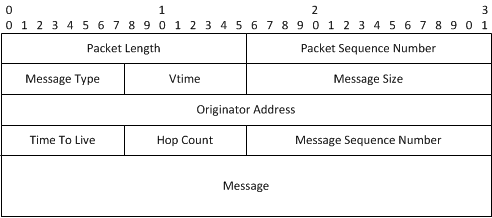
\includegraphics{images/olsr.png}
	\caption{OLSR packet format omitting the IP and UDP headers.}
	\label{fig:olsr}
\end{figure}

\noindent
Because of the regular transmission of control messages, the protocol is sustainable to packet loss which is common in wireless networks. Overhead of control messages in the network is also reduced and redundant control traffic is eliminated by using the MPRs \cite{clausen2003rfc3626}. However, because of the many optimizations added to make the protocol more suitable for ad hoc networks, it also is more complex than e.g. the BATMAN protocol explained in the section below.

\subsection{B.A.T.M.A.N.}\label{batman}
B.A.T.M.A.N., or BATMAN as we will continue to write, is an abbreviation for a "Better Approach To Mobile Ad hoc Networking". It was created with the hope of being a simpler, better and more robust alternative to OLSR. The initial motivation to start the development of the protocol was mainly based on the following reasons \cite{open_mesh}:

\begin{itemize}
\item The OLSR protocol seemed not to be very functional when implemented as specified in \cite{clausen2003rfc3626}. %RFC3626

\item The OLSR protocol depends heavily on the assumption that every node in the network is in possession of almost the same information as all of the other nodes. As they use this information to calculate full routing path to all nodes, the more this information between the nodes differ amongst them, the more likely things like routing loops will occur.
\end{itemize}

\noindent
In order to implement functional OLSR protocol to be used in real-life, the developers found themselves stripping it down removing mechanisms that were initially added to the protocol to optimize it. Eventually the developers had to break compatibility with the protocol defined in \cite{clausen2003rfc3626}. A group of developers felt the OLSR protocol was becoming far to complex and decided develop a routing protocol that was simpler and better, namely BATMAN.
\\\\
BATMAN is, as well as OLSR, a proactive routing protocol where every node has a routing table containing all of the nodes in the network that are accessible via single-hop or multi-hop communication links. The table, which is referred to as Originator List, does however not include the full path to a destination, only the best link-local neighbor towards it. Link-local neighbors are usually referred to as direct neighbors in the BATMAN protocol.
\\\\
Nodes in the BATMAN network build their Originator Lists based on Originator Messages (OGM). These messages are small, containing only a limited amount of information such as version, Time-To-Live (TTL), sequence number, some flags and an Originator Address. The Originator Address is the IP-address of the Originator where the OGM was generated. An Originator is defined in \cite{batman_rfc} as a network interface utilized by BATMAN. Every node in the network periodically generates and broadcasts OGMs for each interface it can communicate through. These messages will be re-broadcasted through the network according to BATMANs forwarding rules until they have reached all the nodes at least once. The format of an OGM is shown in Figure \ref{fig:ogm}.

\begin{figure}[ht]
	\centering
		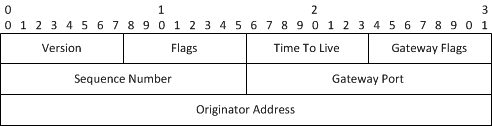
\includegraphics{images/ogm.png}
	\caption{Originator Message (OGM) Format.}
	\label{fig:ogm}
\end{figure}

\noindent
\\\\
The best route to a certain Originator is found by counting the number of OGMs received containing this Originator Address and logging which neighbor it was received from. The best route is thus the link-local neighbor that has the highest count.
\\\\
Details about the BATMAN protocol can be found in the Appendix \ref{appendix_batman}.

\subsection{B.A.T.M.A.N. and OLSR Comparison}\label{batman_olsr_comparison}
One major difference between BATMAN and OLSR is that while OLSR works to reduce the traffic load in the network by restricting which nodes that are allowed to flood, BATMAN does not care about this at all. The reasoning behind this decision is because the protocol was designed to function on unreliable media which is very unstable and can suffer from high packet loss. Thus the flooding of routing information will not saturate the network since most of the packets will be lost due to the lossy media \cite{batman_rfc}.
\\\\
In addition, the nodes in a BATMAN network do not have to calculate the full routing path to all other nodes in the network. By only choosing the next hop towards a destination makes BATMAN a lightweight protocol that quickly adapts to the dynamic topology of ad hoc networks.

\section{Authentication Using Certificates}\label{authentication} % Ny tittel!? authentication and access control / certificates / x.509 certificates
In order to have a restricted ad hoc network there needs to be some form of access control mechanism in place. In traditional computer networks the issue of access control and authentication is usually solved with the use of a hierarchy of trusted third parties, and digital certificates which is associated with every entity participating in the network. A certificate contains information about the entity that defines its identity and rights in the network.
\\\\
This section describes some of the different variants of the X.509 certificates that are used in X.509 Public Key Infrastructure (PKI). 

\subsection{X.509 Long-Lived Public-Key Certificates} \label{LLPKC}
In a Public Key Infrastructure (PKI) the conventional digital certificates are sometimes called Long-Lived Public-key Certificates (LLPKC). They are issued to end-entities by a well-known and trusted Certificate Authority (CA) that digitally signs the certificates with its private key such that it can be verified by anyone in possession of the CAs public key. Each certificate contains the public key of an end-entity and additional data such as subject's public key information, signature algorithm identifier and issuer name \cite{stallings2006cryptography}. 
\\\\
The certificate also contains a validity period of usually months or years which is why they are referred to as "Long-Lived Certificates". This long lifetime entails that a certificate needs to be checked against a Certificate Revocation List (CRL) to ensure that it has not been made invalid whilst still in its validity period. Figure \ref{fig:LLPKC} shows an illustration of a service verifying an end-entity's LLPKC and checking it against a Certificate Revocation List.

\begin{figure}[ht]
	\centering
		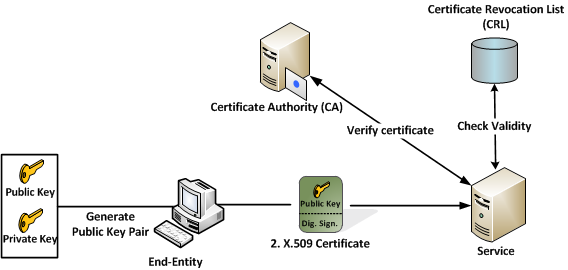
\includegraphics{images/LLPKC.png}
	\caption{An conceptual illustration of the authentication process using LLPKCs.}
	\label{fig:LLPKC}
\end{figure} 

\subsection{X.509 Proxy Certificates} \label{background_pc}
A X.509 Proxy Certificate (PC) is a conventional X.509 public-key certificate containing a critical proxy certificate information extension. The presence of this extension indicates that the certificate is a PC and that it contains one required and two optional fields; pCPathLenConstraint, proxyPolicy and Proxy Certificate Path \cite{tuecke2004rfc3820}.
\\\\
The policy field in the extension can be used to make the PC a Restricted Proxy Certificate (RPC). It contains a field which specifies the appropriate language in which the policy is expressed. This option was intended to provide a finer granularity of control in the rights being delegated.
\\\\
A PC inhabits some of the following properties as described in the Internet standard \cite{tuecke2004rfc3820}:

\begin{itemize}
\item It is signed by an X.509 End Entity Certificate (EEC), or by another PC and is called a Proxy Issuer (PI).
\item An EEC can give certain rights and restrictions to the PC it signs. 
\item It can sign another PC, but nothing else.
\item It contains its own unique public and private key pair.
\item It can be created with any desired lifetime.
\end{itemize}

\noindent
An important feature of the PC is that it is given a unique identity derived from the end-entity who signed it. During the signing the PC may also inherit rights from the PI, subject to the restrictions that are placed on that PC by the PI. Thus the PC has a unique identification which can be used independently and still be associated with the PI who signed the certificate.


\subsection{Other Certificates}
Other variants of the X.509 certificate worth mentioning are Attribute Certificates (AC) and Short-Lived Certificates (SLC). ACs are certificates with a similar structure as a LLPKC, but without a PKC key pair. They contain a set of attributes tied to an identity which is used for authorization and access control decisions. ACs are usually used in association with another certificate that do contain a PKC key pair, such as a LLPKC. The AC may have any validity period desired by the issuer and is usually has a shorter lifetime than LLPKC \cite{farrells2010rfc5755}.
\\\\
The SLCs are modified versions of the traditional X.509 certificates and differ from these mainly because of two characteristics: certificate validity period is no more than 1 million seconds and there is no association between the client and Public Key cryptography (PKC) key pairs \cite{hsu2002intranet}. They were introduced by \cite{hsu2002intranet} with the goal of reducing the costly and difficult key management issues in typical X.509 authentication framework.














\pagestyle{empty}
\cleardoublepage
\pagestyle{fancy}

\chapter{System Design}
\label{ch:design}
\acresetall

This chapter portrays the design for the proposed implementation of the secure
ad hoc network. The design here is based on a functional pro-active ad hoc
routing protocol. The routing is left to the chosen routing protocol, i.e.
\ac{BATMAN}, and the changes made will not affect how the routing is performed.
The system design is an extension of the protocol, which requires nodes to be
authenticated and trusted before being allowed into the network. To strengthen
the system each node also has to verify its identity periodically, or it is
dropped from the network.

\section{Brief Overview}
In this section a short version of the system design is described. It is far
from complete when it comes to explaining the entities, messages being sent,
system states, and why certain choices have been made. This section is
suggested to read through in its entirety just in order to get an overview of
what the system does, leaving the explanations to the subsequent sections.

\subsection{Initial Authentication}
The network setup starts with an out-of-band authentication where a master node,
hereafter \ac{SP}, verifies new nodes. How this is done can be up to the
application, but let us assume that the actors carrying their communication
devices, hereafter nodes, physically meets the \ac{SP} at the scene and verifies
each others' public keys out-of-band.

When a new node is discovered by the \ac{SP} using regular routing announcements
as part of the pro-active routing protocol, the \ac{SP} will invite the new node
to a handshake to establish a trust relationship between the two nodes. In the
invite message the \ac{SP} shares its certificate. If the node can verify the
public key of that certificate, it will request a proxy certificate. If the
\ac{SP} can verify its public key, too, it will issue a proxy certificate with
(possibly) the rights to participate in building the \ac{MANET} by broadcasting
its own and re-broadcasting other trusted nodes' routing announcements.

\subsection{Continuous Authentication}
After being issued with a \ac{PC} the newly authenticated node will periodically
``broadcast'' - unicast to each neighbor - a message containing an ephemeral key
and corresponding \ac{IV}, a pseudo-randomly generated nonce, and a digital
signature over this message. The ephemeral key is encrypted with the neighbor's
public key (hence multiple unicasts instead of an actual broadcast), but the
digital signature is generated using the hash of the unencrypted key and the
other contents of the message.

After sending this signed ``broadcast" to each neighbor, the node and its
neighbors will generate a keystream from the ephemeral key, \ac{IV}, and nonce.
The node will then append two new bytes from this keystream to each routing
announcement, and re-broadcasts of neighbors announcements, sent from this point
forward with a sequence number for the recipient to be able to match this
``extract'' with the keystream at an offset given by the sequence number.

The neighbors accepts a routing announcement if and only if:

\begin{itemize}
  \item the routing announcement is appended with a key extract and,
  \item it matches the sender's keystream at the sequence number offset and,
  \item that sender's sequence number has not been received earlier (replay).
\end{itemize}

This ``key extract'' of the keystream is comparable to regular \acp{OTP} as used
by e.g. online banks and it is important to note that they are not ``connected''
to the routing announcements sent, meaning they do not provide integrity for the
packet.

Note also that each node has its own keystream, and that it shares the message
above, hereafter ``keystream-material message'', with each of its direct
neighbors.

Whenever a routing announcement is forwarded by another trusted node, that
node will replace the one-time password with an \ac{OTP} from its own keystream.
This way every node only checks its direct neighbor for authentication, which is
a design choice. This proposal assumes that because every node is verified by
the \ac{SP} in the first place, all nodes in the network will be able to trust
each other, which also means they will trust their neighbors to properly verify
their neighbors again. This technique also helps prevent a wormhole attack,
which will be discussed later.

%In order for trusted nodes to learn of newly trusted nodes existence, the
%\ac{SP} reularly broadcasts lists containing the id, address and public key of
%each trusted node in the network. This needs to be done, because before
%learning about a new node the other trusted nodes will not accept any messages
%from this node. This means the new node will not be able to exchange its own
%\ac{PC} with other nodes directly - only through the \ac{SP}.

When a trusted node discovers a new neighbor, which is a trusted node in the
network - they first have to exchange their \acp{PC} and verify the signatures
on the certificates. Their knowledge of the corresponding private keys to their
\acp{PC} are only indirectly verified because they need to know the private key
in order to decrypt the ephemeral keys sent with the signed broadcasts by their
neighbors. Each of the two nodes then stores the other's public key, subject
name, id, role, and address in a list called \ac{AL}.

%The list, hereafter \ac{AL}, also adds some \ac{WOT} like capabilities. The
%list is signed by the \ac{SP}, which means the integrity of the list is
%guaranteed by the \ac{SP}. This means that if the \ac{SP} should go offline,
%e.g. it could be out of range, other trusted nodes in the \ac{MANET} can
%continue to broadcast the \ac{SP} on behalf of the \ac{SP} - to ensure all
%nodes in the network know each other. This can be especially important when the
%network grows large and become fully or partially separated and nodes in one
%part may not have learnt of the existence of newly trusted nodes yet. It also
%applies to trusted nodes who have been offline while new nodes have been
%verified, then re-enter the network while the \ac{SP} is offline. [TODO:
%kanskje ref til mitt eget essay?]

After a neighbor is added to the \ac{AL}, the node can then also add the
neighbor to another list, called a \ac{NL}. This list is used to keep
track of current direct neighbors and their current keystreams. While nodes in
the \ac{AL} are kept in that list throughout the lifetime of the network, or
until the lifetimes of the nodes' certificates have expired, a node in the
\ac{NL} is removed when it is no longer a direct neighbor. 

\section{Requirements}
Ad hoc networks have some desired characteristics such as quick and inexpensive
setup and being independent of communication infrastructure, but they also
impose great challenges regarding security. The challenges regarding security
can vary depending the purpose and environment of the network which will be
covered in this section.

\subsection{Scenario}
The design and implementation presented in this thesis is mostly based on an
emergency situation scenario, in which communication infrastructure is
unavailable. This thesis will also reflect on some possible requirements given
by a military application.

If there is a major emergency situation such as an earthquake or tsunami, it is
likely that parts or the entire communication infrastructure at the scene
is destroyed or temporarily down. The remaining communication lines will then
probably be congested, such that little communication actually goes through
[TODO: find a ref].

In this situation, it is of great importance that Emergency Personnel, such as
Paramedics, Firemen, Policemen and the Military, are able to communicate
efficiently and therefore independently of the public communication
infrastructure. They need this network in order to manage the the operation, and
therefore availability is probably the most important trait of this network.
Secondly, they should be able to trust the communication on the network - i.e.
messages sent are from whom they claim they to be.

Also, being able to authorize new actors on the scene, such as Red Cross, can be
critical to the operation. These new actors will probably not have the necessary
authentication tokens, i.e. certificates, required by the authentication scheme
in the network.

\subsection{List of Requirements}
Based on the scenario above these requirements can be extracted and made into
general requirements that needs to be addressed by the system design. The work
presented here is based on several sources, most prevalent being the research
from the OASIS project \cite{oasis_report} \cite{5683058} \cite{nyre2009secure}
and the doctoral project of Eli Winjum carried out at UniK
\cite{ffi_2005_04015}.

\begin{table}[ht!]
	\centering
	%\begin{tabular}{ | l | p{11cm} | }
	\begin{tabular*}{\textwidth}{ | p{5mm} | p{388pt} | }
	\hline
	\textbf{\#} & \textbf{Requirement Description}\\\hline
		R1 & A node must be authorized in order to get full rights in a network \cite{dahill2001secure}, \cite{sanzgiri2002secure}\\\hline
		R2 & A node without a recognized authentication token should be able to become authorized if necessary\\\hline
		R3 & Networks need a master node to handle authentication of new nodes\\\hline
		R4 & Access control (after initial authentication) should work without centralized nodes\\\hline
		R5 & Different networks should be able to collaborate \cite{ffi_2005_04015}\\\hline
		R6 & Only master nodes can decide access policies of users/nodes\\\hline
		R7 & Nodes must not be able to alter their access policies\\\hline
	\end{tabular*}
	\caption{Requirements based upon our simplified and general scenario.}
	\label{tab:our_req}
\end{table}

An early study produced security requirements of ad hoc networks demanding
that the routing logic must not be spoofed or altered to produce different
behavior \cite{dahill2001secure}. R1 is constructed from that requirement.
During the OASIS project, a requirement ensuring different actors such as
police, fire and medical professionals can participate in the network, gives R2
\cite{5683058}.

Because of R2 there needs to be some sort of authority managing the
authentication and access management, which leads to R3. However, verifying
nodes access rights after the fact should be possible even without the
availability (R4) - also a requirement given by the OASIS project.

The doctoral project of Winjum recommends seamless radio coverage over the whole
crisis area, possibly requiring merging or at least collaboration between
different networks, R5.

R7 comes implicitly from R6 because R6 would be useless if regular nodes could
alter their priveleges without the permission of a master or management node. R6
is necessary in this design as no authentication is required prior to the
network setup, and it is therefore no way to know which rights one actor/node
shuold have. As will be discussed in Chapter \ref{ch:discussion} the network
might also be able to recognize authentication tokens, such as long lived
certificates, issued prior to this setup. If this is the case, one might have to
re-evaluate these requirements.

The OASIS had another important requirement which is not covered here, but is
important to mention - there should be mechanisms in place to detect misbehaving
nodes, i.e. already trusted nodes that acts maliciously. This detection is not
covered in this thesis as pointed out in \ref{limit:malicious_behaviour}, but is
nevertheless important to take notice of.

\section{Why use Proxy Certificates?}
\acp{PC}, as described in Section \ref{sect:pc}, are used to delegate
rights on behalf of their issuers. That means that the issuer, i.e. the \ac{SP},
can choose to delegate all or a subset of its rights to the receiver of the
\ac{PC}. This can be very useful in a situation where the nodes themselves are
unable to properly authenticate themselves with their pre-existing \acp{LLPKC}
if the \ac{SP} on the scene has no way to verify their certificates. This can be
true if their certificates are issued by an unknown root certificate (\ac{CA})
or simply if there is no Internet access and the certificate is signed by an
unknown entity (unknown to the \ac{SP}), even if it knows and trusts the root
\ac{CA}. 

In addition, proxy certificates commonly have short valid lifetime compared to
regular certificates, meaning an implementation using proxy certificates does
not necessarily need to implement a certificate revocation scheme, which makes
for less management operations in the management-hostile envirnontment that is
\acp{MANET}. If a certificate is compromised in this \ac{MANET}, the time of
exposure is limited because of the short valid lifetimes on the \acp{PC}.
Regular \acp{LLPKC} on the other hand, could be compromised throughout the
lifetime of the network, or until revocation lists were brought to the scene,
out-of-band or by acheiving Internet access later on.

Also, the \ac{SP} could be interested in giving the node rights the node would
not usually have on this specific scene, depending on the situation. This is
easier to achieve when the \ac{SP} can delegate its own rights. Different nodes
can be given different rights, as long as they are a subset of the SP's rights.
There are countless of different potential rights that can be useful for a
network, given the situation they are used in, and here is a few possible
rights/privileges to give the reader an understanding of the possibilities they
give:

\begin{itemize}
  \item Announce itself - let the \ac{MANET} know of your existence
  \item Re-broadcast other nodes' announcements - reshape the network topology
  \item Announce a gateway - give the \ac{MANET} access to another network
  \item Use the gateway - allow you to communicate outside the \ac{MANET}
  \item Send and receive messages with a defined application - full application
  rights
  \item Only receive messages from a defined application - limited application
  rights
\end{itemize}

The different choices are essentially up to the \ac{SP} managing the network.
One can ask why this is necessary, and again it depends on the application. If
you are setting up a \ac{MANET} on the scene of a disaster to assist emergency
personnel, you could have some actors be able to organize the effort by sending
orders/commands to the other actors, while some actors only are allowed to
receive the orders. In this situation it might be of great importance to know
that only verified nodes are able to give commands, but the importance of
getting this information available outweighs the need to verify the nodes/actors
receiving this information.


\section{Design Overview}
The secure ad hoc network designed here does not change any fundamental workings
of regular ad hoc routing protocols. When nodes have been authenticated and
neighbors have verified their neighbors respectively, the routing annoucements
are generated, broadcasted, forwarded, and handled by the routing protocol
almost as usual. The only addition to the routing protocol is the addition of
one-time passwords (OTP) to the routing announcements, and the handling of said
\acp{OTP}.

The proposed design should work with most pro-active ad hoc routing protocols
operating on the network layer with limited alterations - but this design is
specifically made for the BATMAN \cite{batman_rfc} routing protocol chosen for
its simpler design compared to e.g. OLSR \cite{clausen2003rfc3626} and because
it operates on the third layer of the \ac{OSI} model \cite{zimmermann1980osi}.
Whether this design would work on a link-layer protocol is unknown, and there is
still a discussion whether having routing protocols on the link-layer is a good
thing, as it breaks the layering principles of the \ac{OSI} model
\cite{5680190}. How this design is incorporated, or added, to the BATMAN
protocol will be explained in Chapter \ref{ch:implementation}.

The basic principle of the proposed design is that an authenticated node accepts
other authenticated nodes' routing announcements and forwards them as normal, while
discarding routing announcements from unauthenticated nodes. One or more nodes in the
network will assume a role as master node(s), or a \ac{SP}, with the extra
capability of authorizing new nodes into the network. A special certificate
called a \ac{PC} \cite{rfc3820} will be used for authentication after this
authorization has taken place such that other nodes in the network will be able
to authenticate and accept the new node.

\subsection{Entity Explanation}
Before a simplified example can be given, a few new entities in this design
needs to be explained further. This is the short version, just enough for the
reader to understand the example - the full description of these entities
and why they are necessary will be given later. All of these entities are also
portrayed in Figure \ref{fig:simple_example_entities}. The portrayed entities
will be used as a template for other figures later in this thesis report.

\begin{itemize}
  \item \textbf{\acf{SP}} is responsible for tasks similar to that of a \ac{CA}
  	and has the master role in the network. The \ac{SP} is the entity that
 	authorizes new nodes and signs their \acp{PC}.
  \item \textbf{\acf{PC0}} is a \ac{PC} belonging to a \ac{SP} signed by its
    regular \ac{LLPKC}. This \ac{PC} has a certificate depth of 0, thus we refer
    to it as a \ac{PC0}.
  \item \textbf{\acf{PC1}} is a \ac{PC} signed by a \ac{PC0} (i.e. by the
    private key of the \ac{SP}). All authenticated nodes in one network, has at
    least a \ac{PC1} signed by a \ac{SP} from that network.
  \item \textbf{\acf{AL}} is a list containing the necessary information about
 	all known and authorized nodes in the network. All nodes keep a local copy of
 	the \ac{AL} which they use to authenticate other nodes in the network.
  \item \textbf{\acf{NL}} is a list containing the current trusted direct
    neighbors with a copy of their keystreams used for verifying their routing
    announcements. The \ac{NL} is a subset of the \ac{AL} and a node must be
    found in the \ac{AL} before it can be added to the \ac{NL}.
  \item \textbf{Authenticated/Trusted Node} is a node which has been issued a
    \ac{PC1} from the \ac{SP} and is considered a trusted node in the network.
    This node can take part in sending its own routing announcements and
    forwarding other authenticated nodes routing announcements, i.e. they take
    part in changing the network topology.
  \item \textbf{Unauthenticated Node} is a node which has not yet been
    authorized, or denied access, by the \ac{SP}. They do not possess a
    certificate for which the other nodes can verify, and its routing
    announcements are ignored by other trusted nodes in the network.
\end{itemize}

\begin{figure}[h]
	\centering
  	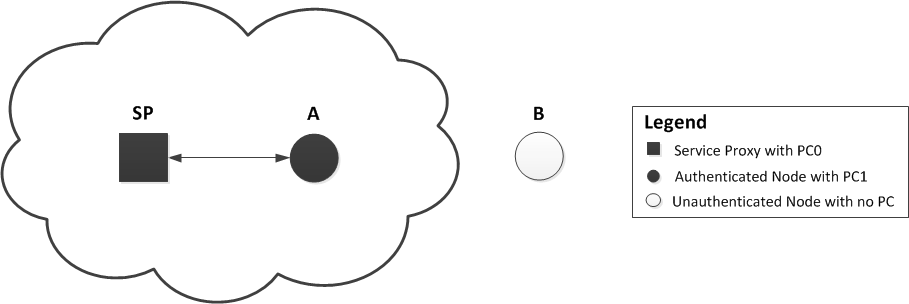
\includegraphics[width=\textwidth]{images/simple_example_entities.png}
  	\caption{Different entities in the Simple Example.}
	\label{fig:simple_example_entities}
\end{figure}

\subsection{Simple Example}
Two nodes are within transmitting range of each other, i.e. they are direct
neighbors. One of the nodes is a \ac{SP} and the other is unauthenticated. The
pro-active ad hoc routing protocol used on both nodes regularly broadcasts
routing announcements, so the two nodes learn of each others' existence - i.e.
they ``discover'' each other. Upon reception of a routing announcement from the
unauthenticated node, the \ac{SP} will invite the node for a handshake. The
invite message contains the \ac{SP}'s \ac{PC0} which assumably the
unauthenticated node is able to verify, possibly based on a prior out-of-band
sharing of public key fingerprints.

After verifying the \ac{PC0}, the unauthenticated node will send a \ac{PC}
request with its own public key. If the \ac{SP} is able to verify the senders
public key (same assumption as above) and the \ac{SP} decides this node should
have access to network, it will create and sign \ac{PC} for this node - i.e. the
node is issued a \ac{PC1}.

%Before the \ac{SP} actually signs the \ac{PC} requested from the
%unauthenticated node, it needs some verification that the node is an actor that
%should be allowed access to the network. The actor will therefore meet the
%\ac{SP} in the field and give its public key fingerprint (out-of-band) so the
%\ac{SP} can verify the incoming public key in the \ac{PC} request as the
%actor's request.

%Using the public key of the \ac{PC1}, the newly trusted node will now create
%and broadcast a signature, and use an excerpt (offset value) from this
%signature in its routing announcements. The signature excerpt is just a value used
%in the following routing announcements, and not the cryptographic signature itself,
%but will be used for recognition. This will be described further later in the
%chapter. The \ac{SP}, recognizing the signature offset value will rebroadcast
%the routing announcements so regular ad hoc routing follows.

When the handshake completes both nodes will add the other node of the handshake
to their \ac{AL} - storing their id, address, unique subject name, role, and
public key. All the steps up to this point is portrayed in the first half of
Figure \ref{fig:simple_example_msc}. As illustrated by the color of the node
circle, the new node (A in the figure) is authenticated after receiving the
issued \ac{PC1}.

Next, both the newly authenticated/trusted node and the \ac{SP} will send one
another a packet called a ``keystream-material message" containing their
current (or new in the case of the trusted node) ephemeral key, \ac{IV}, nonce
value and a digital signature over the hash of these values. Before sending
this message, the ephemeral key part is encrypted with the other's public key
to keep this information secret. Note that the digital signature however, is
computed over the unencrypted key in order to re-use this signature for all
neighbors the node has to send this message to.

Both nodes can now generate the other's keystream (and the new node its own),
hence the name ``keystream-material message'', used to verify the sender of
subsequent routing announcements. These keystreams, address, id, an empty ``last
sequence number'', and an empty sliding window of the other node is then stored
in the \ac{NL}.

%Also upon handshake completion is the generation an \ac{AL}. The \ac{SP} will
%use this list in order to save certain necessary details about the other node,
%such as its address, public key, last signature, and more. Also in this list is
%the corresponding information about the \ac{SP} itself. When the list is
%created or updated it is broadcasted to the network - signed by the \ac{SP} to
%ensure no other node can alter the information about trusted nodes in the
%network.

From this point forward, the two nodes use a two-byte extract of the keystream
as an one-time password and appends it, together with a sequence number (for
finding the correct offset in keystream), to future routing announcements. This
goes for both original routing announcements from the node itself, and when
they forward other trusted nodes routing announcements. The two nodes never
re-use the same extract from the keystream, hence the name ``\acf{OTP}'', and
they use a sliding window stored in their \ac{NL} to keep track of which
extracts they have received from their neighbor. This last part is crucial in
order to be able to drop announcements containing re-used extracts, avoiding
replay attacks. 

Whenever a new node is discovered by the \ac{SP} the procedure above repeats,
and a new addition is made to the \ac{AL} and \ac{NL}. Other previously
trusted nodes will learn the identity of new nodes when they discover the new
node and initiate in a keystream-material exchange, which will be discussed
later.

\begin{figure}[ht]
	\centering
  	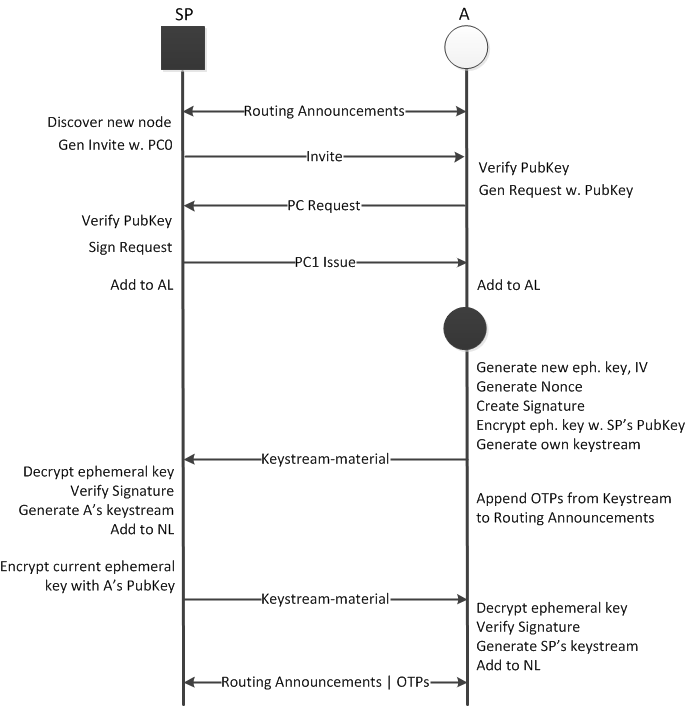
\includegraphics[height=13cm]{images/simple_example_msc.png}
  	\caption{Message sequence chart of the simple example showing authentication
  	  handshake and keystream material sharing between SP and new node A. Routing
  	  announcements at the end contain one-time-passwords (OTP) from keystreams}
	\label{fig:simple_example_msc}
\end{figure}

Figure \ref{fig:simple_example_msc} shows a message sequence chart of the
messages sent between two nodes during the simple example. The second
half portrays the messages sent in a keystream-material message and that
they are added to the \ac{NL} after these have been received, and after
the \ac{AL}-addition. Routing announcements without \aclp{OTP} are sent
periodically throughout the sequence until keystreams are generated, but this
is left out of the figure as they do not affect the nodes. Only the routing
announcements in the beginning and in the end that are appended with \acp{OTP}
are portrayed as they show how the handshake is initiated (by discovery) and
ended after successfully ending the handshake and keystream material sharing.

If a new node enters transmitting range of the two nodes similar messages are
exchanged, as shown in Figure \ref{fig:simple_example_msc_2}.

\begin{figure}[h]
	\centering
  	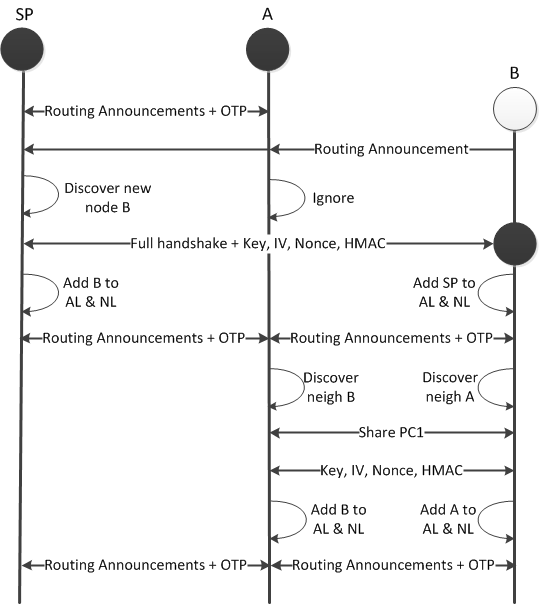
\includegraphics[height=13cm]{images/simple_example_msc_2.png}
  	\caption{Message sequence chart of the simple example showing another node B
  	  attempting to join the network, and the messages between A and B after B
  	  is autneticated by the SP}
	\label{fig:simple_example_msc_2}
\end{figure}

Here we see that after node B has been fully authenticated and started
broadcasting routing announcements appended with its own \acp{OTP}, he and node
A will ``discover'' each other. Up until this point node A has ignored node B's
routing announcements (and forwarded announcements) because they have not been
appended with any valid/recognizable \acp{OTP}.

After they've discovered each other they share their certificates as seen in the
figure. Before continuing they need to verify each other's certificate, which is
to verify the signature on the \ac{PC1}'s up against the public key of the
\ac{SP}.

When both nodes have verified each other's certificates, they send each other
their keystream-material messages, in which they verify each others' signatures
to actually verify each other as the legitemate owners of the certificates. If
they are able to verify each others' signature they will add each other to their
\ac{AL} and \ac{NL}, respectively.

\section{Authentication Phase}
This section is devoted to explain the phases a node goes through before and
when authenticating itself to the network. These phases should be similar for
most network layer pro-active routing protocols as the main trigger of these
phases are the routing announcements sent as per normal operation of any
pro-active routing protocol.

\subsection{Node Discovery}
Upon entering the network area, the node is both unauthenticated and unknown to
the network. Because it uses a pro-active routing protocol, the node regularly
broadcasts routing announcements to be received by any potential node in the
area. At this point an assumption that all nodes are configured with unique
addresses and with the same netmask is done in order to focus on the security
challenges, rather the non-trivial task of assigning addresses in \acp{MANET}
(See Limitations in Section \ref{limit:ip_address_conf}). With this assumption all
nodes within transmitting range of the new node can receive its broadcasts.

\begin{figure}[h]
	\centering
  	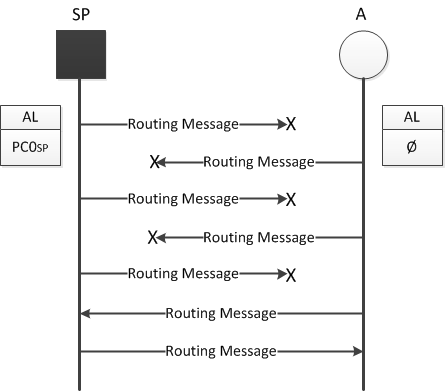
\includegraphics[width=0.6\textwidth]{images/node_states_discovery.png}
  	\caption{Discovery Phase between a \acf{SP} and an unauthenticated node (A)}
	\label{fig:node_states_discovery}
\end{figure}

Simultaneously, the node also listens to other nodes' routing announcements.
Depending on the time interval between the broadcasts and whether the nodes
within each other's transmitting range are asymmetrical, they will discover each
other approximately at the same time.

Figure \ref{fig:node_states_discovery} illustrate the routing announcements
periodically sent by two nodes until they discover each other. One of the nodes
have already assumed the master role and is a \ac{SP} while the other node is
unauthenticated.

The \ac{SP} will have a \ac{PC0} and its \ac{AL} has only one entry - itself.
Note that if it had authorized another node at an earlier point in time (but
within the lifetime of the \ac{PC}) that node's values would also be
represented in the \ac{AL}, even if the node was outside the network at this
point in time (physically).

The new node does not have any \ac{PC} at this point, unless it has a \ac{PC}
issued within and valid only for another network. This is however not covered
here, and it is assumed the node has no certificate at all. The same goes for
its \ac{AL}, or one can rather say it has an empty \ac{AL} - denoted by the
'\O' in the figure.

\subsection{Authentication Handshake}

\begin{figure}[h]
	\centering
  	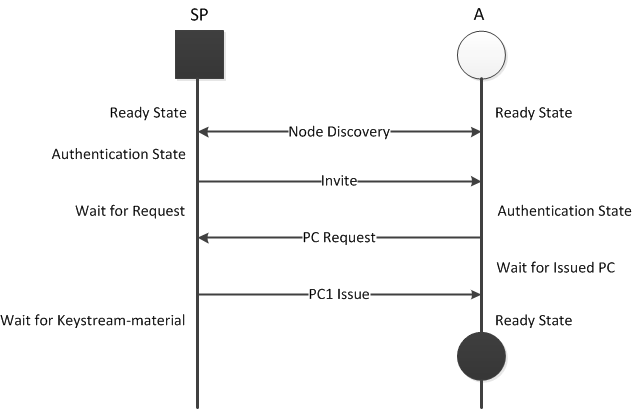
\includegraphics[width=0.6\textwidth]{images/node_states_handshake.png}
  	\caption{Handshake between a \acf{SP} and an unauthenticated node A.}
	\label{fig:node_states_handshake}
\end{figure}

Once the two nodes have discovered each other, the \ac{SP} will enter an
authentication handshake state, while the unauthenticated node will not do
anything. The authentication handshake state of the \ac{SP}, and later of the
other node, does not obstruct regular routing announcements to be sent. The
current state only affects how the \ac{AM} operates, not how the original
routing protocol operates. Actually, the handshake and all other messages and
operations handled by the \ac{AM} is executed in a separate thread and sent
and received using another socket than the rest of the protocol. This is
further elaborated in the next chapter.

Because the unauthenticated node does not enter a new state upon the discovery
of the \ac{SP}, which could just be a regular authenticated node as well, there
will be no deadlock if for some reason the \ac{SP} should never initiate, or
invite to, the handshake. This could happen for a multitude of reasons being
the two nodes looses their connectivity between each other because of the flaky
nature of wireless ad hoc networks, or the assumed \ac{SP} was only a regular
authenticated, trusted, node. From the routing announcements it is not possible
to derive whether a node is simply authenticated, or if it also has master role
capabilities being a \ac{SP}. It is only possible to derive, or rather it seems,
that a node is authenticated in some network or not.

%The unknown node will wait for a predefined amount of time, for it may not ever
%receive a request. The discovery might have been of an authenticated node with
%a \ac{PC1} and not a \ac{SP}, which does not have the rights to authenticate
%new nodes. It might also have been that of a \ac{SP}, but because of the flaky
%nature of ad hoc networks, the two nodes might have become invisible to each
%other before the handshake could be initiated.

While the new node is ``waiting'' for an invite, or simply not doing anything
other than announcing its existence - the \ac{SP} generates an invite message
which is a message containing its \ac{PC0}. The invite will be directly
addressed to the new node, and not broadcasted as regular routing announcements
are. The \ac{SP} will then wait for a certificate request (\ac{PC} Request) for
a short predefined time before aborting the handshake and entering its
ready-state. If the two nodes discover each other once more, the \ac{SP} will
once again try to invite the other node to the handshake. If this fails several
times, the \ac{SP} will eventually ignore the all discoveries of the other node
(based on address) for a predefined time before it tries again.

If the new node is able to verify the SP's public key it will use its public
key pair and generate a \ac{PC} request which it will send back to the \ac{SP}.
This request abides by the rules for making a proxy certificate \cite{rfc3820},
setting the ``Issuer Name'' the same as the ``Subject Name'' from the received
\ac{PC0}, the ``Subject Name'' as the ``Issuer Name'' appended with its own
unique Common Name, which is the hash value of its own public key, and setting
the ``Serial Number'' to the same hash value.

These, and the last step of issuing the \ac{PC1} is shown in Figure
\ref{fig:node_states_handshake}. But before issuing the \ac{PC1} the \ac{SP}
also has to verify the public key received in the request message. As before,
the knowledge necessary to be able to verify the public key is assumed to have been
communicated out-of-band prior to this setup. The \ac{PC1} is appended with the
proxy policies the \ac{SP} seems fit for the node, and then signed with the
\ac{SP}'s private key. After sending the \ac{PC1} to the new node the \ac{SP}
will add the new node to its local \ac{AL} and the new node will, after
verifying the signature on its newly issued certificate, store the issued
certificate for later and add the \ac{SP} to its own local \ac{AL}.

\subsection{Out-Of-Band Authentication}
Above, only brief mention was made to how the initial verification of each nodes
public keys were made. For this purpose, many authentication schemes have been
produced, but when it comes to \acp{MANET}, possibly with no Internet
connection, proper authentication becomes a difficult task. In the discussion
in Chapter \ref{ch:discussion} different schemes will be discussed, but here
only one ``scheme'' is accounted for.

If you have no pre-shared information between the parties involved in the
network, the simplest way to authenticate a new node is to use an out-of-band
authentication. The implementation of such an authentication scheme will be
discussed in the next chapter, and will only be briefly mentioned here.

In the PGP model new users will have to use share their public key fingerprint
with the \ac{SP} physically or through a different communication channel than
the one the authentication process is supposed to secure, and vice versa
\cite{zimmermann1995official}. By doing this, the \ac{SP} can store the
fingerprint and use it to check the received public key in the \ac{PC} request
for authenticity in order to make sure the new node is run by the actual person
he met and verified physically. The new node can similarly verify the \ac{SP}.

To implement this, the application running the routing protocol and the
authentication service could either read a file for ``allowed'' fingerprints, or
simply have user interaction with a pop-up window showing the fingerprint and
asking the user whether to trust the public key or not.

This implementation is relatively simple compared to the rest of the design, so
in this design chapter and in the implementation chapter this part will be
ignored, and rather assume that if you are a direct neighbor of the \ac{SP}, you
are automatically allowed to enter the network and therefore no real
verification of the certificates are done. This must however, be thought through
and most likely changed in a real-world implementation.

\section{Authorized Operation}
%Once a node is authorized and has its own \ac{PC1}, it can send its own routing
%announcements, receive announcements, and forward other nodes' announcements.
%This means that the node is a fully worthy member of the MANET. However, there
%is one thing missing before the node can be verified and verify other nodes
%(than the \ac{SP}) - i.e. it has to learn the public key and address of all its
%neighbors.

%Figure \ref{fig:node_states_authorized} shows the authorized node receiving
%an \ac{AL} Update from the \ac{SP}. This message contains the full \ac{AL} list
%and lets the newly authorized node learn the public key and address of
%potential other nodes in the network. The list is broadcasted by the \ac{SP}
%periodically to make sure all nodes in the network know and trust each other.

%\begin{figure}[h]
%	\centering
%  	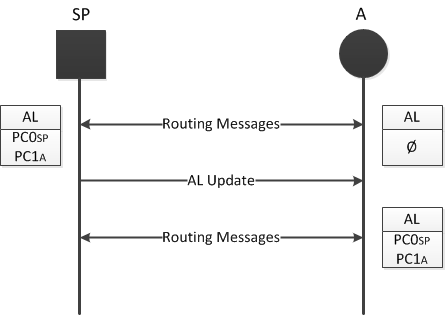
\includegraphics[width=0.5\textwidth]{images/node_states_authorized.png}
%  	\caption{Normal operation between a \acf{SP} and an unauthenticated node
%  	(A)including an \ac{AL} Update message.}
%	\label{fig:node_states_authorized}
%\end{figure}

When a node has been issed a \ac{PC} and become a trusted node in the network,
it is almost ready to take part in the sending and forwarding of routing
announcements. But before a node can take part in the routing in the network, it
has to be able to append one-time-passwords to its routing announcements, and to
verify other nodes' one-time-passwords as it receives routing announcements from
them.

\subsection{Keystream generation}
The \acp{OTP} are actually smaller extracts of larger keystreams shared
between direct neighbors in the network. When a node started its routing
protocol daemon and before discovering the \ac{SP} in the previous step, it
generates a high entropy pseudo-random master key and a regular pseudo-random
\ac{IV}. The master key needs high entropy to be as random as possible, because
the security of this design relies on this key to both be secret and not
guessable.

When the node is ready to share its keystream for the first time, the node will
generate a new ephemeral key by encrypting $K_{ephemeral} =
E_{K_{master}}\{i\}$ where $i = 1,2,3\ldots$ and a corresponding \ac{IV}
generated in the same manner as the previous \ac{IV} for the master key. In
addition a large nonce is generated with a pseudo-random function, also in the
same pseudo-random fashion as the \acp{IV}. To elaborate, this pseudo-randomness
does not need strong randomness with a high entropy like the master key, it only
needs to be (with high probability) different for each time.

With the current ephemeral key, generated with $i = 1$, \ac{IV} and nonce, the
node can now generate its first keystream to be used as \acp{OTP} for its
routing announcements. The keystream is generated by encrypting the nonce with
the ephemeral key multiple times, each time extending the size of the
keystream. Each encryption is a full ``Cipher-block chaining'' AES encryption,
i.e. each encryption step referred to here (and later) are actually multiple
encryptions using the AES-CBC mode.

In the first encryption (full AES-CBC) the supplied \ac{IV} is used, while in
the next iterations a 16 byte extract of the output from the previous encryption
(ciphertext) is used as \ac{IV}. To explain, this is basically a \ac{CBC} mode
encryption of multiple AES-CBC blocks. To lessen any confusion a figure to
illustrate this is in order. Figure \ref{fig:keystream_generation} shows
process assuming the ephemeral key, IV and nonce has already been created.

\begin{figure}[h]
	\centering
  	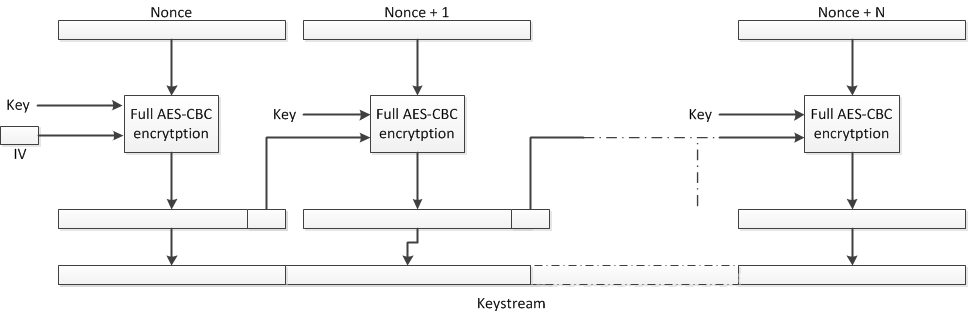
\includegraphics[width=\textwidth]{images/keystream_generation.png}
  	\caption{Keystream generation using a nonce value N times with a simple plus
  		one multiplication. Each nonce will go through full AES-CBC encryption. The
  		keystream output is all the generated ciphertexts appended. The different
  		sizes between IV and nonce are not correct, the nonces are about 60 times
  		larger in size than the IVs.}
	\label{fig:keystream_generation}
\end{figure}

In the figure there are some boxes marked with ``Full AES-CBC encryption''. This
is meant to illustrate that within each of those boxes there is a full AES-CBC
encryption taking place, with multiple steps according to the standards of
AES-CBC. The reader should also notice that as the ciphertext output of each of
those boxes are much larger than the AES block size, therefore only an AES block
size extract at the end of the ciphertext is used as an \ac{IV} for the next
encryption step, instead of the whole ciphertext which would usually be done in
CBC as there the ciphertext corresponds to the correct block size.

\subsubsection*{Keystream Sharing}
Now, before this keystream can be used to authenticate routing announcements,
the node will have to share the keystream with its direct neighbors. This is
done by sending all the material necessary for the neighbor to create the
keystream themselves and signing the message with your private key. I.e. the
node will have to send the ephemeral key, \ac{IV} and nonce to its neighbor.
Here it is crucial that the key stay secret between the neighbors, therefore
the node will have to encrypt the ephemeral key with its neighbors public keys
and send a unicast message with the keystream material to each one of them. The
details around sharing the keystreams will be further explained in the
following section regarding all messages sent in the network
(\ref{sect:am_messages}).

\subsection{Using \acfp{OTP} from Keystream}
Once the keystream has been shared with the neighbors, the node will begin to
extract smaller chuncks of the keystream and use an \ac{OTP} for each
routing announcement it generates itself, or forwards from other trusted
neighbors. In addition to the \acp{OTP} appended to the announcements,
the node keeps a counter, or sequence number, to keep track of which
\ac{OTP} it has used in order not to use the password twice.

Similarily the node will have to both verify the correctness of the \acp{OTP}
received in announcements from its trusted neighbors, and that it has not been
received before. If the password has been received before the annoucement needs
to be dropped, and assumed is part of a replay-attack. If the node would have
accepted re-using of one-time-passwords, an attacker could listen and record
valid one-time-passwords and re-use them with false routing information in
order to disrupt the routing in the network.

How to check for replayed one-time-passwords is further elaborated in the next
chapter, but simply put a sliding window recording the last announcements are
used, setting a bit value to true if an announcement with the corresponding
sequence number (keystream sequence number, not from original protocol) has been
received, and zero if not.

\subsection{Discovering New Neighbors}
Up until this point, the node only had only discovered the \ac{SP} and after the
authentication handshake shared their keystream material in order to be able to
trust each others routing annoucements. Because of the trust mode being used in
this design, each routing annoucement from the \ac{SP} are trusted, even if they
are re-broadcasts (forwarded by the SP) originating from other nodes not yet
known to the new node. This means that the routing table of our node could
possibly fill up with unknown nodes, reachable through \ac{SP}. To have all
data streams go through the \ac{SP} however, would be less than ideal. If some
of those nodes are direct neighbors of our node, they should be able to
communicate directly.

Therefore a discovery mode of other trusted (by the network at least) nodes
needs to be handled. Until now, if you received any routing announcements
from an unknown neighbor you would have dropped the packet. After becoming an
authenticated node, the node will now instead engage in a exchange of \acp{PC}
with the other neighbor. If the neighbor sends you a \ac{PC} with a signature
of the \ac{SP} which you are able to verify, you will add the node to your
\ac{AL} and send him your \ac{PC} - if you have not sent it already.

The verification of the ownership of the \ac{PC} is not performed before
receiving the keystream-material message which occurs soon after sharing
\acp{PC}. As a remainder the keystream-material message is signed with the
private key of the sender. Therefore, assuming the nodes has not been
compromized, the ownership of the neighbors are verified by checking the
validity of said signatures.

\section{Detailed Entity Description}
This section describes the different entities in greater detail. How they are
used and why they are present is some of the questions that will be answered.

\subsection{\acf{PC}}
In a scenario where actors try to communicate with each other, without the
Internet or other communication infrastructure available one cannot depend on a
\ac{PKI} for authentication of the actors. One needs the option of being able
to verify actors physically (out-of-band) and then issuing them an
authentication token to be used during this scenario. This is where the
\aclp{PC} comes in handy. Regular \acp{EEC} should not be used for issuing new
certificates, per the RFC2459 \cite{rfc2459}, and even if one did use them for
this purpose there is no definition on how to handle topics as path validation
and such.

Using \acp{PC} this issue can be handled in a well-defined manner. The field
``pCPathLenConstraint'' is used for constraining the depth of the certificate
chain below the \ac{PC} itself. I.e. if a \ac{PC} has a pCPathLenConstraint of
zero, the \ac{PC} cannot issue any other \acp{PC} itself, while if the 
pCPathLenConstraint value is one the \ac{PC} can be used to issue new \acp{PC}
which again will have a pCPathLenConstraint of zero, and so on.

For our scenario, the pCPathLenConstraint value should never exceed one, or else
it will once again be difficult to handle path validations. Every node trying to
verify a \ac{PC} need to know the issuer of the certificate directly, and not
indirectly through root \acp{CA} as is possible if you have a \ac{PKI}.

A \ac{PC} is almost a regular certificate, except for some values that are
forbidden to use, some values that are required to use, and some values that
must be used in a well defined way \cite{rfc3820}. Below are the
fields that are included in this system design:
\begin{itemize}
  \item Subject Name: $<$Isser Name$>$ + ``CN: $<$SHA-1(Public Key)$>$''
  \item Issuer Name: $<$Subject Name of Issuer$>$
  \item Serial Number: ``$<$SHA-1(Public Key)$>$''
  \item X509v3 Extensions:
  \begin{itemize}
    \item Key Usage: ``Digital signature, Key encipherment''
    \item ProxyCertInfo:
    \begin{itemize}
      \item pCPathLenConstraint: $<$0 or 1$>$
      \item proxyPolicy: 
      \begin{itemize}
        \item policyLanguage: ``id-ppl-anyLanguage''
        \item policy: ``Role:$<$sp or authenticated$>$,Routing:$<$full or limited$>$,Application:$<$full or limited$>$''
      \end{itemize}
    \end{itemize}
  \end{itemize}
\end{itemize}
Per RFC3820 (\cite{rfc3820}) the subject name has the constraint that it
``should be unique amongst all Proxy Certificates issued by a particular Proxy
Issuer''. The modal verb ``should'' used in this requirement is used in order
to ease this requirement so that a method creating a unique name with a high
probability, but not provable uniqueness, should be accepted. Therefore using a
SHA-1 digest of the public key used by the node is regarded as ``good enough'',
or ``unique enough''.

The same requirement is true for the serial number, and allows the serial number
to be the same as the subject name except for the ``CN:'' prefix.

The specifications requires the ``Digital signatures'' value for the ``Key
Usage'' extension because a \ac{PC} can be used to sign the keystream material
messages. ``Key encipherment'' is also necessary in this extension because other
neighbors need to use your public key to encrypt their ephemeral keys when they
want to share their keystream with you.

The ``policyLanguage'' field is set to the default value, leaving the
language used in the policy field later to be handled correctly by the
application, rather than being universally understandable.

Finally, the last field called ``policy'' might be of greates interest. This
field explains what rights the given \ac{PC} has for this design. Three values
have been defined for use in this design:

\begin{itemize}
  \item Role - Node's role in the network
  \item Routing - Whether the node can partake in the routing
  \item Application - Whether the node has access to the application layer
\end{itemize}

These values are specific to this design, and might not be of any desire in
other applications. The first value, ``role'', is used to declare which role the
node has been given. It can be ``sp'' which means the node as administrative
rights in the network, or ``authenticated'' meaning the node is trusted by the
\ac{SP} and should be trusted by all other nodes in the network.

The ``routing'' value can be ``full'' or ``limited''. If it is full the node is
able to generate and broadcast its own routing announcements, and forward its
trusted nodes routing annoucements. This means the node partakes completeley in
the network and might be placed in a path between two nodes in the network. The
``limited'' value is used so a node can become an end-node, but not a node in a
path between other nodes. I.e., it can send its own routing announcements, but
it cannot forward other nodes' routing annoucements. If a node with limited
rights does forward other nodes' announcements they must drop the packets. In
addition, a detection system of misbehaving nodes should pick up this as
potentially malicious behaviour, but this is not being implemented as previously
explained in Limitations (\ref{limit:malicious_behaviour}).

The last value, ``application'', is used to declare whether the node should have
access to the upper layers and being able to use the applications running on top
of the \ac{MANET}. This restriction is useful if one has special devices in the
field only used to route/forward packets in the network, acting similar to
routers in the regular Internet, but not being able to e.g. respond to
application requests. Nodes which does not use the application layer will reside
in each nodes routing tables, but should not show up as available nodes on the
upper layers.

\subsubsection*{\acf{PC0}}
A \acl{SP}'s \ac{PC0} would typically be filled with the values in the
\ref{tab:pc0_values}. For illustration, this \ac{PC} has been issued by the
\ac{SP}'s regular \ac{LLPKC} issued by NTNU.
\begin{table}[h]
	\begin{tabularx}{\linewidth}{ | l | X |}
		\hline
 		\textbf{X.509 Field} & \textbf{Value}\\\hline
		Subject Name & C=NO, L=Trondheim, O=NTNU, OU=ITEM, CN=Espen, CN=$<$SHA-1(Public Key)$>$ \\\hline
		Issuer Name & C=NO, L=Trondheim, O=NTNU, OU=ITEM, CN=Espen \\\hline 
		Serial Number & $<$SHA-1(Public Key)$>$ \\\hline 
		Key Usage & Digital signature, Key encipherment \\\hline 
		pCPathLenConstraint & 1 \\\hline 
		policyLanguage & id-ppl-anyLanguage \\\hline 
		policy & Role:sp,Routing:full,Application:full \\\hline 
	\end{tabularx}
	\caption{Values in \acf{PC0}}
	\label{tab:pc0_values}
\end{table}
The zero in the PC0 abbreviation is used to indicate that the certificate is at
a depth of zero and has a pCPathLenConstraint of one which means that the
\ac{SP} is allowed to issue new \acp{PC}, but that the children of the \ac{PC0}
cannot be used to issue new \acp{PC} again. 

\subsubsection*{\acf{PC1}}
If the PC0 above was used to issue a regular PC1 to an authenticated node, the
values might look like the ones in Table \ref{tab:pc1_values}.
\begin{table}[h]
	\begin{tabularx}{\linewidth}{ | l | X |}\hline
 		\textbf{X.509 Field} & \textbf{Value}\\\hline
		Subject Name & C=NO, L=Trondheim, O=NTNU, OU=ITEM, CN=Espen, CN=$<$SHA-1(PubKey(SP))$>$, CN=$<$SHA-1(Public Key)$>$ \\\hline
		Issuer Name & C=NO, L=Trondheim, O=NTNU, OU=ITEM, CN=Espen, CN=$<$SHA-1(PubKey(SP))$>$ \\\hline
		Serial Number & $<$SHA-1(Public Key)$>$ \\\hline 
		Key Usage & Digital signature, Key encipherment \\\hline 
		pCPathLenConstraint & 0 \\\hline 
		policyLanguage & id-ppl-anyLanguage \\\hline 
		policy & Role:authenticated,Routing:full,Application:full \\\hline 
	\end{tabularx}
	\caption{Values in \acf{PC1} if issued by the \ac{PC0} above.}
	\label{tab:pc1_values}
\end{table}
The interesting part here is too see that the subject name contains the full
subject name of the issuer in addition to the hash value of the public key used
in the PC1. Note also that the pCPathLenConstraint now denies the owner to issue
other acp{PC} using this certificate.

\subsection{\acf{SP}}
The term \acl{SP} was coined by Dr. Lawrie Brown \cite{lawrie:technotes}.
\acp{SP} are used in place of regular \acp{CA} for \acp{PC}. The \ac{SP}
determines whether a node should be issued a \ac{PC} and if so which policies to
attach. The \ac{SP} drastically distinguishes itself from regular \acp{CA}
because it breaks the hierarchical model usually associated with \acp{CA} when
they are part of a \ac{PKI}.

A \ac{SP} can also be part of a \ac{PKI} (issued a regular public key
certificate), but because of our scenario, it can be difficult or impossible to
verify its regular certificate. Therefore, this verification is handled
out-of-band instead.

In this design, the \ac{SP} is a master node which decides which nodes can get
access to the network and if so what rights they have. The \ac{SP} assigns its
\ac{PC0} with all the rights which might be useful for the current scenario, so
that it can delegate those rights to other nodes when issuing them \acp{PC1}. In
a larger network, there would typically be more than one \ac{SP}

\subsection{\acf{AL}}
The \ac{AL} is a local list that each trusted node including the \ac{SP} in
the network maintain to keep track of which nodes they knows and the necessary
information about them. An \acl{AL} stores these values for each node they have
met and shared their \acp{PC} with:
\begin{table}[h]
	\centering
	\begin{tabular}{| l |}\hline
 		\textbf{\acl{AL}}\\\hline
		ID\\\hline
		Address \\\hline
		Role \\\hline 
		Subject Name \\\hline 
		Public Key \\\hline  
	\end{tabular}
	\caption{\acf{AL} content}
	\label{tab:al_content}
\end{table}
Both the ``ID'' and ``Subject Name'' fields stored for each node are unique, so
one could ask why one needs the ID field when the unique subject name is used in
accordance with RFC3820 (\cite{rfc3820}). The answer is actually quite simple,
it is easier and safer to look for the ID value when going searching in the
\ac{AL} because it is a number while the subject name value is a text.

For all nodes but the \ac{SP} in the network, the first entry in the \ac{AL} is
the \ac{SP}. This is only natural because the \ac{SP} is the first node they
start to trust as it is the one node that actually issued their \ac{PC} in the
first place. To illustrate this, if you go back to the two nodes' \acp{PC} in
Tables \ref{tab:pc0_values} and \ref{tab:pc1_values} and you have a third node
with these two nodes in its \ac{AL}, the \ac{AL} might look like Table
\ref{tab:al_content_3_nodes}.
\begin{table}[h]
	\centering
	\begin{tabularx}{\linewidth}{| l | X |}\hline
 		\textbf{Fields} & \textbf{Values}\\\hline
 		\hline
		ID & 45251\\\hline
		Address & 192.168.57.1\\\hline
		Role & SP\\\hline 
		Subject Name & C=NO, L=Trondheim, O=NTNU, OU=ITEM, CN=Espen, CN=$<$SHA-1(2AF2E5C75C\ldots)$>$\\\hline
		Public Key & 2AF2E5C75C\ldots\\\hline
		\hline
		ID & 1341\\\hline
		Address & 192.168.57.45\\\hline
		Role & Authenticated\\\hline 
		Subject Name & C=NO, L=Trondheim, O=NTNU, OU=ITEM, CN=Espen, CN=$<$SHA-1(2AF2E5C75C\ldots)$>$, CN=$<$SHA-1(DA912BC9F5\ldots)$>$\\\hline
		Public Key & DA912BC9F5\ldots\\\hline  
	\end{tabularx}
	\caption{An \acf{AL} in a network with three trusted nodes.}
	\label{tab:al_content_3_nodes}
\end{table}
Note that the arbitrarily chosen values for e.g. the Public Key here does not
show a complete size public key. Also, the public keys stored in the \ac{AL}
would be stored as their real binary values, and not Base64-encoded as the table
portrays. In the subject name there is a common name part with ``SHA-1()'' -
meaning that the content here would actually be the sha-1 digest of the content
inside the brackets.

\subsection{\acf{NL}}
The \acl{NL} is a list each node in the network maintains to keep track of its
current neighbors and the necessary information about them.
\begin{table}[h]
	\centering
	\begin{tabular}{| l |}\hline
 		\textbf{\acl{NL}}\\\hline
		ID\\\hline
		Address\\\hline
		Sliding window\\\hline 
		Last sequence number\\\hline 
		Keystream\\\hline
		Number of wrong OTPs\\\hline
		Time keystream received\\\hline
	\end{tabular}
	\caption{\acf{NL} content}
	\label{tab:nl_content}
\end{table}
Table \ref{tab:nl_content} shows the content fields for each entry in the
\ac{NL}. The first important thing to recognize is that the node entries in the
\ac{NL} are not necessarily the same as the node entries in the \ac{AL}. When a
node meets new neighbors and looses old direct neighbors (which are still in
the network nevertheless) new entries are added while old entries are removed.
This means also that the index in the two lists are not the same - and here's
where the use of the ID field comes in. Whenever both lists has to be looked up,
the ID field is used in order to retrieve the same node from both lists.

Besides the ID and the address the keystream field should be expected to reside
in the \ac{NL} by the observant reader. If not, this is where the keystreams of
your neighbors are stored, and updated each time you receive a new
keystream-material message from said neighbor. There are four other fields too
however, which might not be expected by the reader. These fields play an
important part in mainstaining this list and most importantly - replay attack
protection.

First, the ``Time keystream received'' field stores the time (in seconds) when
the last keystream from this neighbor was received. The \acl{AM} regularly
checks to see if it has not received keystreams from nodes in the \ac{NL} for
some time, and purges all entries older than a defined timeframe. This is mainly
to keep the \ac{NL} up to date and short, as the keystreams take up memory
storage.

The remaining three fields are quite more interesting, as they are used for
replay attack protection.

\subsubsection*{Sliding Window}
The sliding window is a bit array of 64 bits size \cite{peterson2007computer}.
This window is used in order to decide whether a routing announcement should be
allowed through to the routing protocol, or if the \ac{AM} should block and
drop the announcement. Each bit in the window can either be 0 or 1, and it is
used to declare whether an \acf{OTP} already has been received (bit set to 1)
or not (bit set to 0).

The ``last sequence number'' field is used to indicate the last, or highest,
keystream sequence number of the last routing announcement received from this
neighbor. If the last sequence number is X, then the sliding window corresponds
to the the sequence numbers between X-63 and X. I.e. the sliding window shows
whether an \ac{OTP} from this range has been received or not.

For a node to accept a routing annoucement from a direct neighbor (which is in
its \ac{NL}), the following MUST be true:
\begin{itemize}
  \item the \ac{OTP} sequence number must either be inside the sliding window,
  	or higher than the current last sequence number, and
  \item the same sequence number must not have been received before, i.e. the
  	bit at its sliding window position must be 0, and
  \item the \ac{OTP} must match the keystream at this sequence number offset.
\end{itemize}
Note that when a new keystream is calculated for a neighbor, the old sliding
window and last sequence number are replaced so the same sequence numbers can be
used again.

The last field, ``Number of wrong OTPs'', is increased whenever a received
routing announcement fails the checks above, i.e. if its an too old sequence
number, it has been received before, or if the \ac{OTP} does not match the
expected \ac{OTP} from the keystream. If this value is too high, the node will
delete the neighbor entry from its \ac{NL} and request a new keystream-material
message.

\section{\acf{AM} Messages}
\label{sect:am_messages}
This section describes the different messages sent within, or modified by, the
\ac{AM} extension. This includes how they are created, what payload they
contain, if and how the information is secured from malicious actors, and
finally to whom and how often they are sent during normal operation.

\subsection{Authentication Handshake}
The authentication handshake describes which messages are sent while
authenticating a new node to the network. The handshake is triggered by an event
where the \ac{SP} discover a new and unauthenticated neighbor node.

\subsubsection*{Node Discovery}

TODO: ICH BIN HIER!

Node discovery is not actually a part of the handshake itself, but it is the
event that triggers the handshake and is described here to make the context more
clear to the reader.

As described earlier each node stores a local copy of the \ac{AL} and a direct
neighbor node list. Whenever a trusted node receives a routing announcement from
a new neighbor, i.e. a node which is not in the direct neighbor list, the
trusted node needs to check the \ac{AL} to see if the node is a trusted node. If
the node can be found in the \ac{AL} the trusted node will request the signature
of the node and store it alongside the address of the node in its neighbor list.

If the node is an unknown node however, regular trusted nodes, i.e. nodes issued
with a \ac{PC1}, will discard the announcement and go on with its other
operations. \acp{SP} will initiate an authentication handshake in the same
event.

\subsubsection*{Handshake Invite}

\subsubsection*{\acf{PC} Request}

\subsubsection*{\acf{PC} Issue}

\subsubsection*{ACK ?}
Maybe share the signature (rand+aes-key) in this ack?



\subsection{Routing Announcement Authentication}
In the ideal world every routing announcement broadcasted on the network would
be signed for authenticity and integrity, but for our scenarios and \acp{MANET}
in general the world is far from ideal.

One huge limitation is packet size - because each routing announcement is
broadcasted throughout the network, and the network in our case is a higly lossy
one, one needs to constrain the packet size or else all the throughput in the
network would be used on routing announcements. The decision was therefore made to
include only a small value of 16 bits to deduce node authentication and to
assume packet integrity.

Later in Section \ref{sect:routing_auth_solution} the idea  behind this
solution is discussed, partly defending why this solution was chosen, and partly
what limitations this solution has compared to more traditional ways.

\subsubsection*{Signature?? Message}

The idea is similar to other \ac{MAC} solutions [TODO: find ref] except only a
special packet sent periodically is verified - instead of each routing announcement.
This packet contains a pseudo-randomly generated value, a temporary symmetric
key generated from the master key, and signed hash value of the packet.

TODO: mention master key here or earlier??

The neighbor receiving the packet first computes a message digest, hash, of the
first part of the packet, and decrypts the signed hash value contained in the
packet and checks to see if they are identical. If so, the neighbor trusts this
packet to be from an actual trusted neighbor.

The packet cannot be broadcasted, because there is no shared group key between
all nodes in the network, but has to be unicasted to each of the direct
neighbors - encrypted with their public keys.

\subsubsection*{Extended Routing Announcements}

The routing announcements are appended with 16 bits of the \ac{MAC} code, which
is the pseudo-random value encrypted with the symmetric key. For each routing
announcement there is a counter, which tells the receiving neighbor at which
offset of the \ac{MAC} value the 16 bits belong to.

Depending on how fast the \ac{MAC} is exhausted, the sender can instruct its
neighbors to create a bigger value based on the same pseudo-random value. For
example the nodes can be instructed to generate a \ac{MAC} ten times the size of
the pseudo-random value - easily done by incrementing and encrypting the random
bytes ten times.

TODO: Add figure showing these messages, and explicitly the 16 bits extracted
from the mac\ldots

For each routing announcement a neighbor receives, he checks the 16 bits at the
given offset of the self-generated \ac{MAC} and if it matches - he assumes the
message is from his trusted neighbor. If any packet contains 16 bits extract
that does not match the \ac{MAC} at the given offset, the packet will be
regarded untrusted and dropped.

\begin{figure}[h]
	\centering
  	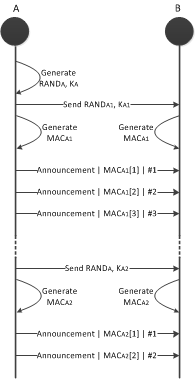
\includegraphics{images/mac_ogm_msc.png}
  	\caption{Node A peridically generates a new pseudo-random value and a
  	corresponding symmetric key which it shares with its neighbor B. Node A use
  	an extract of a generated MAC of this value in each of its routing
  	announcements hereafter.}
	\label{fig:mac_ogm_msc}
\end{figure}

\subsubsection*{REWRITE OVER\ldots}
In a typical MAC algorithm you send a message appended with a MAC value. Then
the receiver takes the message, creates his own MAC value and compares it with
the received MAC value\ldots 

In this solution, the first message, find a name for it!, will contain a message
(pseudo-random value), WITHOUT the MAC value. (It must also be encrypted and
signed.,..). 

The MAC value is instead sent with the routing announcements, instead of with
the initial message itself.

Will be rewritten later.

\subsection{\acf{AL}}

\subsubsection*{\acf{AL} Update}

\subsubsection*{\acf{AL} Single Row Update}

\pagestyle{empty}
\cleardoublepage
\pagestyle{fancy}

\chapter{Implementation}

The security additions to the BATMAN protocol are mostly implemented in the
\ac{AM}, but some alterations had to be made in other parts of the code as well.
This chapter is devoted to explain what have been done as to achieve the design
goals, but the code itself is found in Appendix \ref{chapter_source_code}.

\section{Proof of Concept Solution with Dedicated Socket}
Based on the implementation done in the previous project where we proposed a
proof of concept solution with no actual cryptographic authentication scheme -
this section describes how that solution was extended to use a separate socket
in order to achieve the performance needed, as discussed in the project.


\pagestyle{empty}
\cleardoublepage
\pagestyle{fancy}

\chapter{Testing \& Results}
\label{ch:testing_results}
\acresetall

In this chapter two tests are described and their results presented and
discussed. The two tests measure and compare the time performance in two common
stages for both the original implementation of BATMAN, and the extended version
proposed and implemented in this thesis.

\section{Test I - Initialization Phase}
The ``initialization phase'' is the setup phase between two or more nodes trying
to create a network. With the original implementation of BATMAN this phase only
consist of two stages; namely discovering a neighbor node, and deciding to add
the node as a direct link, or ``last-hop'' per BATMAN terminology, in its
routing table.

With the proposed design and implementation from this thesis, two more stages
are added. After the discovery, the authentication handshake stage and the
keystream sharing stage are conducted before the last stage where BATMAN adds
the node as a new direct link in its routing table.

The time measured here in this test is the time between the first discovery of a
new neighbor, until that node is added to the routing table.

\subsection{Hypothesis}
With the modified version of BATMAN proposed in this thesis, one should observe
a small extra delay in the setup of the network, compared to the original
BATMAN protocol. This extra delay should however, not be significantly higher,
i.e. it should be relatively constant and at no time should any linear increase
in delay be observed.

\subsection{Setup}
\begin{figure}[h]
	\centering
	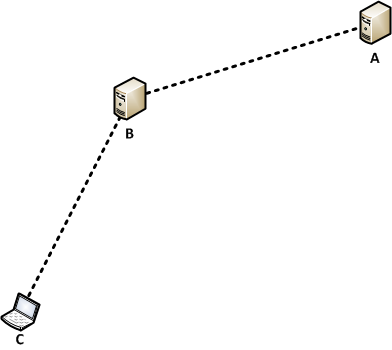
\includegraphics[width=0.5\textwidth]{images/setup_test_1.png}
	\caption{Physical network layout used in test 1. When using the modified version node B acts as the SP of the network}
	\label{fig:setup_test_1}
\end{figure}

Figure \ref{fig:setup_test_1} presents the setup of the test machines used to
conduct this first test. Node A and B are stationary boxes while node C is a
laptop. Their hardware specifications are described in Appendix
\ref{appendix:lab_setup}. The reasoning to use a different hardware for node C
is the need to create distance in the network, and that outside the ethernet
subnet for which the two other nodes were connected to, it would be easier to
use a laptop during setup. In the next test, this laptop is yet again moved
further away.

An important feature to notice about how these nodes were set up is that node A
and C are outside each other transmitting range, meaning they need an
intermediate node to route their packets to and from each other. Node B is
conveniently placed with almost equal distance to each of the two other nodes.

The landscape the nodes are setup in is a typical office landscape, with varying
obstructing materials such as concrete, wood, and glass. A more ideal setup
would naturally be outdoors, as the network is intended for, but with the lack
of mobile nodes and time this became out of the option.

\subsection{Procedure}
In order to get the same behavior each run for the modified version, each run
had to be run discretely, i.e. after each run the daemon was shut down and
restarted. This way each run will include all four stages explained above:
discovery, authentication handshake, keystream material sharing, and routing
table update. This was also done on the original implementation, even though
there are no authentication steps in between, but in order to have the exact
same procedure each time.

For each run, these steps were followed:
\begin{enumerate}
  \item Start Node A and C
  \item Wait and make sure both nodes are stable
  \item Start Node B
  \item When both node A and C are discovered and added to routing table kill
  all daemons
  \item Record the log from node B
\end{enumerate}
These steps were taken 10 times in order to have a reasonable data set and
average. Then for each of the 10 logs, record the time between the first routing
announcement received from a node, until both nodes have been added to the
routing table.

\section{Test II - Route Convergence}
The next test is to check how quick route convergence the protocols deliver when
a path between nodes in the network changes. As with the previous test, a
node running the original protocol needs to discover a new direct neighbor and
add it to its routing table. In addition, it will have to receive not only the
neighbors own routing announcements, but also routing announcements it has
forwarded on behalf of its own direct neighbors. When this happens, the node
receiving these re-broadcasts determines new routes to possibly new nodes -
adding them to its routing table.

Additionally, nodes using the modified BATMAN protocol needs to share
their keystream material with their new direct neighbor before adding that
neighbor in their routing table. When this has happened, any re-broadcasted
routing announcements from that neighbor is accepted and paths to those nodes
are updated, or added if new nodes. Note also that no authentication handshake
or sharing of certificates are mentioned, as they are assumed to have been
shared prior to this route change.

\subsection{Hypothesis}
As before, a small and relatively constant (mathematical term) extra delay is
expected when running the modified version of the protocol compared to running
the original. As the keystream material sharing only occurs between the direct
neighbors, it should only happen once during one run and not for each of the new
nodes added by the path through the direct neighbor - i.e. there should be no
linear increase in convergence time even if multiple new nodes are added to the
routing table with paths through a new neighbor.

\subsection{Setup}
\begin{figure}[h]
	\centering
	\subfloat[Initial Position - D out of range of C]{\label{fig:test_2_1}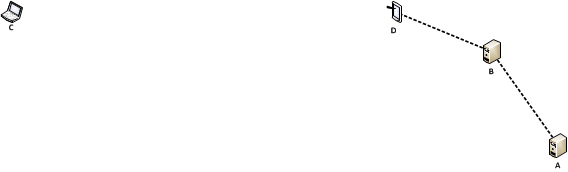
\includegraphics[width=\textwidth]{images/setup_test_2_1.png}}
	\\
	\subfloat[``Connected Position'' - D within range of C]{\label{fig:test_2_2}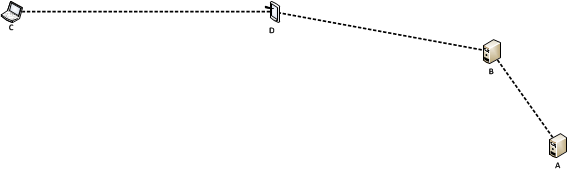
\includegraphics[width=\textwidth]{images/setup_test_2_2.png}}
	\caption{Physical network layout used in test 2. The Laptop (node C) is moved further out of range and is periodically rejoining the network when a Tablet Pc (node D) is moved within range. When using the modified version node B acts as the SP of the network}
	\label{fig:setup_test_2}
\end{figure}

For this test a new mobile node was needed. As Figure \ref{fig:setup_test_2}
shows the Laptop, or node C, from the previous test is moved much further away,
so far in fact the newly added Tablet Pc, node D, needs to place itself with
approximately the same distance to node B as to node C in order for node C to
take part in the network.

Node A and B is positioned at the same place as in the previous test, in the
same office landscape. The line of sight is, however better between node B and
D, and between D and C. Their line of sighs are only obstructed by a single wall
with huge windows.

\subsection{Procedure}
With this test running each of the 10 iterations discretely would be too time
consuming, because it would have meant that the Laptop (node C) would have to be
physically moved inside the transmitting range of node B for each run. Instead
the laptop was only started within the range of the other nodes, in order to be
authorized and share certificates with the other nodes (only node B and D was
necessary) and then moved to its position long outside the transmitting range of
the rest of the network. After this ``initial setup'' plus some minutes to
clear the neighbor lists, these steps were followed:
\begin{enumerate}
  \item Walk node D in between node B and C
  \item Wait until the whole network has stabilized
  \item Walk node D back out of node C's range
  \item Wait until BATMAN has cleared node D from other nodes routing tables,
  and node D has cleared all other nodes from its routing table
  \item If modified version is used, make also sure node D is removed from the
  \ac{NL} (should be before routing tables are cleared)
\end{enumerate}
These steps were repeated 10 times for both implementations. The records used
from this test are from the logs of node C. The convergence times measured
are the time between each time a new neighbor (node D) is discovered by BATMAN,
and until a path to the furthermost node (A) is added to the routing table.


\section{Results}
In this section the results from the two tests above are presented and discussed
in terms of how they perform compared to the hypotheses. In both tests there
were only a dataset of 10 trials, which given the variance shown below does not
provide a statistical significant result. However, the first test shows good
indication that the modified protocol behaves as expected, while the results
from the seconds test are more ambiguous. The results below are presented in
graphs, while all of the numerical results and the test logs are found in
Appendix \ref{appendix:test_results}.

\subsection{Initialization Phase}
Figure \ref{fig:results_test_1} presents the first test's results for both the
original and modified version of BATMAN. The two graphs shows the time in
seconds on the y-axis and the trial/run number on the x-axis. The two colored
lines on the graphs shows the results from first neighbor discovery until the
first neighbor is added to routing table (green line) and until both nodes are
added to the routing table (red line).

\begin{figure}[h]
	\centering
	\subfloat[Original B.A.T.M.A.N.]{\label{fig:test_1_original}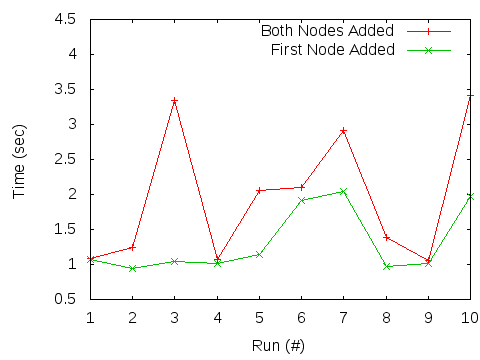
\includegraphics[width=0.5\textwidth]{images/test_1_original.png}}
	\subfloat[Modified B.A.T.M.A.N.]{\label{fig:test_1_secure}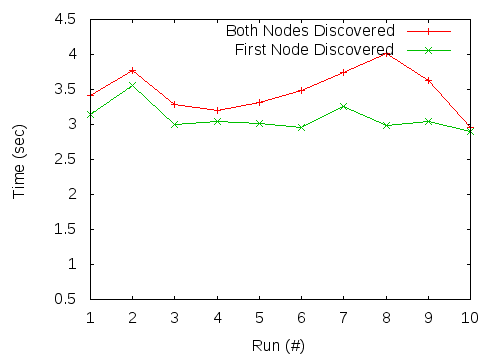
\includegraphics[width=0.5\textwidth]{images/test_1_secure.png}} 
	\caption{In a network of three nodes, the time spent by the \ac{SP} from its first neighbor discovery and until both neighbors are added to its routing table.}
	\label{fig:results_test_1}
\end{figure}

The results from the original protocol, shown in Figure
\ref{fig:test_1_original}, shows high variance in the time needed to add one and
two nodes to the routing table. For 7 out of 10 ``first nodes'' the time needed
is relatively equal, being about one second. For both nodes to be added however,
there are much more variance - varying from the best possible time, i.e. equal
to adding one node, and up above 3 times longer than adding one node. As this is
from the original implementation of BATMAN, this thesis will not try to explain
why this behavior is observed, nor does the author know exactly why either.

Figure \ref{fig:test_1_secure} shows the results from the modified version
proposed in this thesis. These results indicates that the behavior of the
modified version seems to correlate with the behavior expected from the
hypothesis. A seemingly constant of about two seconds seems to be added to the
process of adding both nodes to the routing table. 

Another interesting observation is that the time variance seems to be much less
from that of the original version. This might be because the authentication
handshake and the keystream sharing happens in a separate thread from the
regular BATMAN operations, meaning the BATMAN protocol continuously receives
routing announcements to process while the \ac{AM} handles its part. The idea
being that while the \ac{AM} thread runs the BATMAN thread ``gets ready'' to do
its part of the job.

\subsection{Route Convergence}
The results of the second test is shown in Figure \ref{fig:results_test_2}. In
this figure, the axes are the same as in the figures above: y-axis shows the
time in seconds, and the x-axis shows the trial run. The red line shows the
performance of the original implementation, while the green line shows the
modified.

\begin{figure}[h]
	\centering
	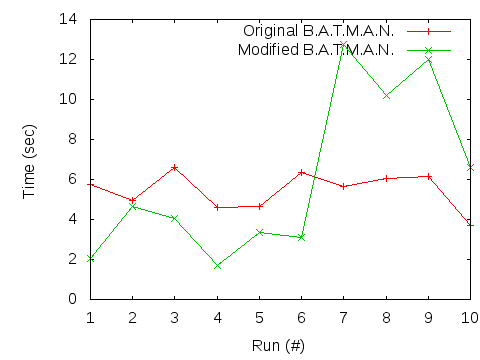
\includegraphics[width=0.8\textwidth]{images/test_2.png}
	\caption{Routing path convergence time observed by a distant source node to another sink node in the network. The source node is only sporadically connected to the network through a mobile intermediate node.}
	\label{fig:results_test_2}
\end{figure}

As indicated earlier, this test's results are somewhat unclear. While the
results using the original implementation seems relatively uniform, with only
about 1 second variance, the results from the modified implementation is highly
irregular.

Looking through the logs from this test one thing become apparent. With
different hardware on the different nodes in the network, their wireless cards
send at different strengths meaning while one node can receive packets from a
``stronger node'', the packets sent might not be received by the other nodes.

The BATMAN protocol messages (routing announcements) are sent quite often,
depending on the number of re-broadcasts being sent, meaning the time from when
a node is within transmitting range and until its broadcasts are received by
nodes within its transmitting range will be quite short. The \ac{AM} messages
however, was mostly tested in an ideal environment where most packets were
received, so this was not properly accounted for. Therefore, if a routing
announcement from a ``stronger node'' is received by a ``weaker node'', the
weaker node might send its keystream material without the other node receiving
it.

Re-transmitting mechanisms based on guessing that the receiving node has not
received the \ac{AM} messages are in place, but as the mechanism wait until it
believes the other node has not received, instead of knowing it instantly. This
can of course be managed adding ACK'ing to each \ac{AM} message, which was not
added initially because of the wish to minimize overhead. This however, might
have to be re-evaluated.

Another thing to notice is how multiple trial runs using the modified version
actually performed better than the original version. This is impossible to
explain talking about the design and implementations themselves, but is probably
most accurately explained in the terms of external environment.

In this test, one major factor is the movement of the Tablet Pc, or node D. This
movement is not perfect, and will vary in speed, timing, and accurate position
for each run. As self-generated routing announcements are only generated once
every second, a difference in almost two seconds can be seen based on the
difference in distance each run. Also, the original implementation only starts
its whole neighbor discovery after an original (self-generated/produced)
routing announcement is received from a new neighbor. The \ac{AM} is triggered
on the first routing announcement received from that new neighbor, even if that
announcement is a re-broadcast from another node in the new neighbor's network.


\pagestyle{empty}
\cleardoublepage
\pagestyle{fancy}

\chapter{Discussion}
\label{ch:discussion}
\acresetall

\section{Modified Routing Announcements Vulnerability}
The design was changed a bit during implementation, and with limited time some
parts did not make it to the implementation These things needs to be addressed
before the system can be used in a real world scenario. There are two attacks
that the system are still vulnerable to, namely the \emph{wormhole attack} and
the \emph{suppress replay attack}.

Because the routing announcements are unencrypted and the one-time-passwords
are just appended after the messages, these packets can be altered using the
following two attacks. In this section the two attacks are first explained, and
then the section goes on to describe possible solutions for both attacks.

\subsection{Wormhole Attack}
In a wormhole attack, see Figure \ref{fig:wormhole_attack}, an attacker does not
need to know the keystream of a node in order to send that node's routing
announcements. If you look at the figure from the background chapter you have a
network of trusted nodes in green, and two malicious nodes in red. 

Assume the two attackers, M1 and M2, want to disrupt the network topology by
having node B believe node A (and vice versa) is a direct neighbor. Assuming the
out-of-band wormhole in the figure is a faster route between node A and B than
the ``real'' route through the network, M1 can simply forward the announcements
from A to M2. Then M2 does the same, except he also needs to spoof his network
and link layer addresses. When B receives the routing announcement from M2, he
believes it is from A and that A is a new direct neighbor.

Now B will ask for A's keystream-material, and M2 and M1 will forward this
request to A, which will dutifully reply with his keystream-material. Note that
M1 needs to spoof B's addresses here, as well as forwarding B's routing
announcements. When B receives the keystream through the wormhole, he is now
able to verify the routing announcements also sent through the wormhole, and
soon will this route take priority in his routing table as a strong direct link
instead of going through other nodes in the network to reach A.

TODO: MSC FIGURE VISER DETTE

This attack only distorts the network topology, but notice that because the
routing announcements' integrity are not protected, and the content is not
encrypted, the attackers can possibly do greater damage by altering the content
of the message. By altering the content, they could possibly generate fake
re-broadcast announcements announcing untrusted nodes, possibly connecting a
whole network of malicious nodes to this trusted network. This alteration is
not actually a wormhole attack, but it is fair to say that the wormhole attack
opens up to a variety of other attacks, such as alteration of packet, dropping
of packets etc.

\subsection{Suppress Replay Attack}
Another attack which is possible due to the fact that the one time passwords are
not ``connected'' to the routing announcements in any way is the suppress replay
attack. Suppose an attacker is able to jam the signals for a very short time,
only enough to distort the main payload of the routing announcement, while the
one time password and its sequence number are kept intact.

The trusted receiver of this distorted packet will ignore it, because he will
not understand the meaning of the packet. The attacker on the other hand, knows
that the following un-corrupt data is a valid one time password and its sequence
number from the sender's keystream.

Because the original recipient of this packet did not understand the destroyed
packet, he will not know that this \ac{OTP} is already used, and if the attacker
wishes to create a false routing announcement he can now do this and append the
\ac{OTP}, which will be accepted by the original recipient. Note that also here
the attacker needs to spoof the addresses of the original sender of the
announcement which he partly jammed.

\subsection{Possible Solution to the Suppress Replay Attack}
A possible solution to the suppress replay attack, is to ensure message
integrity in addition to the authentication. The basic idea would be to create
and append a message digest to the announcement while using the keystream to
encrypt the message, e.g. by using a strong stream cipher.

There is one great pitfall to this idea, however. Because the routing
announcements are often identical to each other, the attacker might be able to
do a known plaintext attack, being able to first recreate the message digest,
and depending on the stream cipher just XOR the announcement and digest with the
encrypted message, revealing the keystream used by the stream cipher. If this
message was in any way blocked from reaching the intended recipient, the packet
could be changed and XOR'ed with the retrieved keystream and sent to the
recipient, which would trust this packet.

One possible way to avoid this problem would be to add some randomness to the
``known part'', namely the original announcement. If the announcement is e.g.
appended with a part of the senders keystream (\ac{OTP}) before creating the
message digest, the attacker would not be able to recreate the full plaintext
(including digest) and would therefore not be able to find the keystream used by
the stream cipher.

The reader might raise another question, regarding the length of this random
part added to the announcement before creating the digest. One major factor
here is time, and time it takes for an adversary to find the random part (collision).
The time is however very restricted. The sliding window used to avoid replay
attacks is only 64 bits long, and in the worst case (best case for adversary)
there are only two legitimate nodes in the network. If this is the case, each
node will send two announcements every second (BATMAN protocol) meaning the
window of opportunity for the attacker is only 32 seconds. For each extra
legitimate node in the network this window drastically closes. The length of the
random part used for the digest should therefore be strong enough withstand 32
seconds of brute-force guessing attack.

Note that it might not be wise to send the whole message digest because the
announcement sizes would become very large. This might be truncated as well, but
when designing this the time needed to find a collision for a truncated digest
needs to be addressed as well.

\subsection{Possible Solution to the Wormhole Attack}
This attack vector is very difficult to to protect against. With the solution
above, many attacks dependent on the wormhole attack are thwarted because of
packet secrecy, integrity and authentication. However, the solution does not
hinder an attacker from replaying the exact same packets through a wormhole, in
order to alter the network topology. There has been a lot of research to find a
good solution to this attack, but most solutions are aimed towards stationary
networks and not \acp{MANET} \cite{raoteapproaches}.

One possible solution as pointed to by the article above is the use of
``location aware guard node'' and graph theory \cite{poovendran2007graph}
\cite{lazos2005preventing} to detect wormholes. The idea is that if you have
special nodes spread out in the field at fixed points, where none of these nodes
are within each other's transmitting range, one should never be a neighbor of
more than one node at a time. If you receive direct packets from two nodes
within a very short time frame, there might be indications that there's a
wormhole in place replaying one of the special nodes' announcements.

\section{Key Usage}
In the fields of information security and cryptography it is not considered a
good practice to use the same keys for different type of tasks such as
encryption for confidentiality and signing for integrity and authenticity. It is
argued that using only one key for different purposes brings a single point of
failure to the design. While this is true, sometimes the benefits of having
single key for these purposes are greater than the risk. In the proposed design
the same public key pair is used to digitally sign keystream-material messages
as well as when encrypting (with the recipient's public key) the symmetric keys
in the same messages. In addition, the \acp{SP} use the same key to sign other
nodes' \acp{PC}.

The benefits of only having a singe public key pair for each node in the network
is simplicity in the design. When it comes to the possible vulnerability if the
one key is compromised, the lifetime of each key which is bound by the
relatively short lifetime of \acp{PC} makes the window of opportunity for misuse
of this key short and damage low.

\section{Future Work - Extending the System Design}
The specialization project \cite{bowitz_graarud} that preceded this thesis
mentioned other important features the secure ad hoc network implementation
should have. The things mentioned in this thesis' system design are actually
implemented, but there are still much more that should be added if this system
should be used in real life emergency situations.

In this section some important features which should be added, or at least
studied, are mentioned. They do add more complexity to the system, so it is
probably better to do a complete security and performance analysis on this
thesis' proposed design before adding these features.

\subsection{Initial Authentication with Long-Lived Public Key Certificates}
One limiting factor in the system design is the need for an out-of-band
initial authentication. With this limitation, every actor in the emergency
scenario needs to manually verify his or her identity to the network management
handled by the \ac{SP}. With many actors, which would be typical in a large
emergency situation like a natural disaster, this process might take up valuable
time from the actual emergency work - which contradicts the whole meaning of
setting up the \ac{MANET} at the scene in the first place.

Now, if an actor has possession of a regular \ac{LLPKC} which the network
\ac{SP} is able to verify, this should be allowed without the need of an
out-of-band authentication. After the \ac{SP} has verified the certificate, he
can now issue the the actor a proxy certificate, signed by him so that all nodes
in the network are able to verify the new node's identity.

The question of whether the \ac{SP} is able to verify the \ac{LLPKC} is not
necessarily easy to answer. If the \ac{SP} trusts the identity and knows the
public key of the issuer of the actor's certificate, he is able to verify that
this actor was trusted with this identity (and rights) at some time. However, it
does not mean this is true anymore - the certificate might have been revoked.

In the absence of Internet access, \acp{CRL} might not be available to the
\ac{SP}. If this is the case, an evaluation of what to do with the actor has to
be done. Ideas that comes to mind might be to issue a very short lived \ac{PC},
maybe with limited rights, to the actor's node so that it can start working now,
but has to re-authenticate later when \acp{CRL} has been brought to the scene
either out-of-band or by setting up Internet access. If no \ac{CRL} is ever
brought to the SPs attention, he might want to require an out-of-band
authentication later.

Either way, as this does not have to happen in the same out-of-band fashion as
the proposed design in this thesis requires, one could also allow the
authentication to happen even if the actor is not a direct neighbor of the
\ac{SP}, but is connected through other nodes in the network. While in this
implementation regular trusted nodes drop the announcements from new
unauthenticated nodes, they could rather tunnel the announcement directly to
the \ac{SP} and have the authentication handshake go through them.

\subsection{Network Merging}
For this implementation to be really useful for emergency services, which will
consist of different types of actors and organizations, the implementation
should support merging of multiple ad hoc networks. For example, if paramedics
set up their own network, and firefighters arrive with their own network,
co-operation between these networks should be supported.

Figure \ref{fig:scenario_networks} (from the specialization
project \cite{bowitz_graarud}) shows a possible scenario when a large emergency
situation such as a natural disaster has happened. The figure portrays 4
organizational actors, i.e. police, firefighters, paramedics, and the military,
which all run their own networks. Some of the networks co-operate through the
use of gateways, such as between the police and the other actors, and the
paramedics and firefighters co-operate by merging their networks.

\begin{figure}[h]
	\centering
  	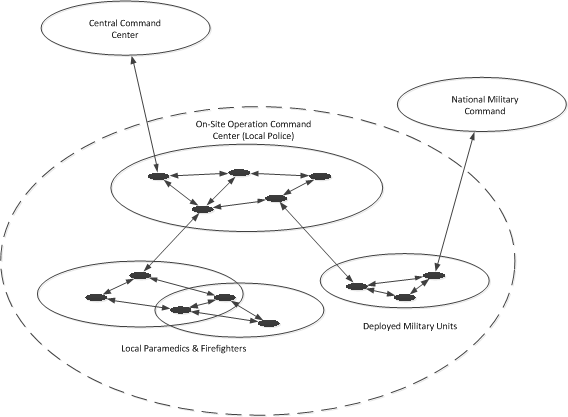
\includegraphics[width=\textwidth]{images/scenario.png}
  	\caption{Scene from scenario with actors from multiple organizations.}
	\label{fig:scenario_networks}
\end{figure}

Choosing whether to merge two networks or not is mainly a security issue. Some
actors might have higher security concerns than others, e.g. military units does
not trust the other actors to merge with their networks, but they might still want
to communicate with them. This can for example be handled by having certain
gateway nodes being allowed to communicate with nodes outside the network in a
controlled manner.

\subsubsection*{Full Merging}
A \emph{full merging} means that two or more separately built and maintained
networks completely merge so that each node in each of the networks receive
all the routing announcements being sent within the networks. What this
basically means is that the different networks become a single network.

The transition to from multiple to one network is not easy. Up to this point
the assumption has been that there is only one management node called \ac{SP}
in the network. This will now change. With multiple networks merging into one
there will be multiple \acp{SP} managing the access control of the network. In
the next section having multiple \acp{SP} is discussed in greater detail.

There is one more major factor which needs to be addressed with full merging of
networks, namely how access control is defined. One now needs to assume that the
\acp{SP} either use the same policy languages to define what rights a node have
been attributed with, or that they have a way of translating these policy
languages so that they can be uniformly understood. For instance, in Section
\ref{subsect:detailed_pc_descr} three special attributes and their values were
used as an example of how a policy might look like:

\begin{itemize}
  \item Role - Node's role in the network
  \item Routing - Whether the node can partake in the routing
  \item Application - Whether the node has access to the application layer
\end{itemize}

Now, these attributes would seem to make sense in most applications of this
system design, but some implementations might even have more attributes. Their
values might also be different, because different networks might have different
needs, for instance the 'role' attribute might have different values depending
on what kind of elements are present in the network. For instance, one network
might have the ``location aware guard nodes'' mentioned earlier in the network
for wormhole protection, while other network do not. With two such different
networks, full merging might not be feasible, but with smaller differences the
obstacles might be manageable.

\subsubsection*{Limited Merging}
\emph{Limited merging} is a completely different technique than the one
described above, and probably easier to implement. With limited merging of two
or more networks, the networks stay autonomous with their own (possible)
hierarchy, set of rules, management nodes, and so on. What constitutes the
merging is that at least one node in each network is set up with gateway
capabilities, which can broadcast the existence of another network to the nodes
inside its own network.

Rules on the application layer must necessarily still be looked at, as they
should work over the different networks, but routing rules and other access
controls can stay hidden between the networks.

\subsubsection*{Internet Gateway}
Similar to limited merging, a node in a network may be given gateway capabilities
to announce Internet access to the network. Because all nodes belong to the same
\ac{MANET} and the management is consistent within this one network, this
capability should be relatively easy to implement. The only thing the reader
should notice is that the policy field within the proxy certificates of the
nodes can now be used to declare whether the node should have Internet access or
not by adding an \emph{Internet attribute} to the policy.

\subsection{Multiple Service Proxies}
Whenever full merging of two secure and managed MANETs happen as described above
two \emph{or more} (!) SPs will end up in the same network (the emphasis on more
is used because one network might have more than one SP). This would be a
challenging task to overcome, for these networks are inherently flat, or
non-hierarchical. Decision making in the network after this point would be
difficult if one network (or specifically one SP) sees itself as more important
than the other.

It is probably better to say that for two networks to fully merge, they should
see themselves as equal counterpart where no network has more rights than the
other, and therefore the \acp{SP} have the same rights as each other. This means
that nodes issued by one \ac{SP}, or said differently one SP's children, are
equally trusted by all other nodes in the network, depending on the restrictions
set in their \acp{PC} of course.

If all the \acp{SP} in the network are considered ``equal'', then they are all
equally trusted to issue new nodes and introduce them to the network. The major
requirement missing for this scheme to happen is that all nodes in the network
now needs to know the public keys for all SPs.

It is likely that not all nodes in the network will ever become a direct
neighbor and therefore not receive the other SPs' \acp{PC0}, but they will meet
nodes signed by those SPs. A way around this problem is to have each \ac{SP} to
once in a while broadcast a digitally signed list to all its children nodes
containing the identities (unique subject names) and public keys for all other
trusted \acp{SP} in the network. Because this list is signed by a known
\ac{SP}, you are able to verify the authenticity of this list and therefore
implicitly verify and trust all nodes issued with PCs from the other SPs.

\section{Experience with OpenSSL}
The experience with OpenSSL has been a challenging one. There is little
documentation available, and only on some segments of the library. Many
functions being used in the implementation of this thesis are undocumented, or
at least not in a freely available documentation. Not to be confused, you can
find most OpenSSL functions in their documentation, but most of those functions
are not explained, many do not explain output and input to functions, and many
functions have unclear names making it a game of ``guessing'' which functions to
use.

Most of the implementation has been understood by looking at a few available
examples online at different sites, some demos within the OpenSSL libraries,
and by asking the online community. For reference, I would personally recommend the
community at \emph{Stack Overflow}\footnote{\url{http://stackoverflow.com}}
rather than the OpenSSL mailinglists\footnote{\url{openssl-dev@openssl.org}}
\footnote{\url{openssl-users@openssl.org}} which have not answered any
questions I raised.

When I've had enough time I've documented the OpenSSL functions used in my
implementation, which can hopefully help someone planning to further implement
on this design, or other designs with similar functionality.

TODO: mention why ECC not used, problems with ECIES algorithm

\pagestyle{empty}
\cleardoublepage
\pagestyle{fancy}

\chapter{Conclusion}
\label{ch:conclusion}
\acresetall



\pagestyle{empty}
\cleardoublepage
\pagestyle{fancy}

\bibliographystyle{alpha}
\renewcommand{\bibname}{References}
\bibliography{ref}
\addcontentsline{toc}{chapter}{References}

\pagestyle{empty}
\cleardoublepage
\pagestyle{fancy}

\appendix
\chapter{Source Code}
\label{appendix:source}
\acresetall


\definecolor{darkgray}{rgb}{0.95,0.95,0.95}
\lstset{
	language=c,
	basicstyle=\footnotesize,
	numbers=left,
	numberstyle=\footnotesize,
	stepnumber=0,
	numbersep=5pt,
	backgroundcolor=\color{darkgray},
	showspaces=false,
	showstringspaces=false,
	showtabs=false,
	frame=single,
	tabsize=2,
	captionpos=b,
	breaklines=true,
	breakatwhitespace=false,
	escapeinside={\%*}{*)}
}

%\section{BATMAN}
%
%\subsection{batman.h - struct bat\_packet}
%\lstinputlisting[frame=tb]{source_code/batman.h}
%
%\subsection{batman.c - batman()}
%\lstinputlisting[frame=tb]{source_code/batman.c}
%
%
%\section{SCHEDULE}
%
%\subsection{schedule.c - excerpt}
%Line numbers indicate where the code is added to the original source code.
%\lstinputlisting[frame=tb]{source_code/schedule.c}
%
%
%\section{AM}
%
%\subsection{am.h}
%\lstinputlisting[frame=tb]{source_code/am.h}
%
%\subsection{am.c}
%\lstinputlisting[frame=tb]{source_code/am.c}


%\pagestyle{empty}
%\cleardoublepage
%\pagestyle{fancy}

%\chapter{IRC Chat Logs}
\label{chapter_irc_logs}
\acresetall

\definecolor{darkgray}{rgb}{0.95,0.95,0.95}
\lstset{
	language=c,
	basicstyle=\footnotesize,
	numbers=left,
	numberstyle=\footnotesize,
	stepnumber=0,
	numbersep=5pt,
	backgroundcolor=\color{darkgray},
	showspaces=false,
	showstringspaces=false,
	showtabs=false,
	frame=single,
	tabsize=2,
	captionpos=b,
	breaklines=true,
	breakatwhitespace=false,
	escapeinside={\%*}{*)}
}


\section{Previous Sender Field}
%\lstinputlisting[frame=tb]{irc_logs/03_26_2011_#batman.txt}

%\section{BATMAN}
%
%\subsection{batman.h - struct bat\_packet}
%\lstinputlisting[frame=tb]{source_code/batman.h}
%
%\subsection{batman.c - batman()}
%\lstinputlisting[frame=tb]{source_code/batman.c}
%
%
%\section{SCHEDULE}
%
%\subsection{schedule.c - excerpt}
%Line numbers indicate where the code is added to the original source code.
%\lstinputlisting[frame=tb]{source_code/schedule.c}
%
%
%\section{AM}
%
%\subsection{am.h}
%\lstinputlisting[frame=tb]{source_code/am.h}
%
%\subsection{am.c}
%\lstinputlisting[frame=tb]{source_code/am.c}


\pagestyle{empty}
\cleardoublepage
\pagestyle{fancy}

\chapter{Lab Setup}
\label{appendix:lab_setup}


The computers used in the lab was setup with the following hardware:

\begin{itemize}
\item Intel Core 2 Duo 2.83 GHz processor
\item 4 GB memory
\item Atheros AR5413 802.11abg NIC
\end{itemize}

\noindent
Further, they are setup with Ubuntu 10.4 (Linux Kernel 2.6.32-25-generic-pae) and ath5k drivers for the wireless interfaces. The network interface is configured as follows:


\begin{lstlisting}[frame=tb]
/etc/network/interfaces

auto lo
iface lo inet loopback

auto wlan0
iface wlan0 inet static
address 10.0.0.X
netmask 255.255.255.0
pre-up ifconfig wlan0 down
pre-up ifconfig wlan0 hw ether XX:XX:XX:XX:XX:XX
pre-up iwconfig wlan0 mode ad-hoc essid BATMAN channel 3

auto unicast
iface unicast inet static
address 10.0.0.X
netmask 255.255.255.0
pre-up brctl addbr unicast
pre-up brctl addif unicast wlan0
pre-down ifconfig unicast down
post-down brctl delif unicast wlan0
post-down brctl delbr unicast
\end{lstlisting}

\noindent
\\
To install batmand, run the following as root user:

\begin{lstlisting}[frame=tb]
make
make install
make clean
\end{lstlisting}

\noindent
\\
For running the batman daemon on the test nodes, we ran the following script as root user:

\begin{lstlisting}[frame=tb]
ifconfig wlan0 up
batmand wlan0
batmand -cd 4
killall batmand
ifconfig wlan0 down
\end{lstlisting}

\noindent
\\
For reducing the transmitting power in test III and IV we ran the following as root user:

\begin{lstlisting}[frame=tb]
ifconfig wlan0 down
iwconfig wlan0 txpower 7
ifconfig wlan0 up
\end{lstlisting}




\pagestyle{empty}
\cleardoublepage
\pagestyle{fancy}

\chapter{Test Results}
\label{appendix:test_results}
\acresetall
\section{Numerical Results}
This sections presents the actual numerical results the graphs in Chapter
\ref{ch:testing_results}, and their means and variances.

\subsection{Test I - Original BATMAN}
\begin{table}[h!]
	\centering
	\begin{tabular}{| l || p{24mm} || p{22mm} | p{22mm} || p{20mm} |  p{20mm} |}\hline
 		\textbf{\#} & \textbf{First OGM Received (s)} & \textbf{First Route Added (s)} & \textbf{Last Route Added (s)} & \textbf{Time to Add One (s)} & \textbf{Time To Add Both(s)}\\\hline
 		 1 & 0.35 & 1.42 & 1.44 & 1.07 & 1.09\\\hline
 		 2 & 0.41 & 1.35 & 1.65 & 0.94 & 1.24\\\hline
 		 3 & 0.18 & 1.22 & 3.52 & 1.04 & 3.34\\\hline
 		 4 & 0.75 & 1.77 & 1.82 & 1.02 & 1.07\\\hline
 		 5 & 0.18 & 1.33 & 2.24 & 1.15 & 2.06\\\hline
 		 6 & 0.02 & 1.94 & 2.12 & 1.92 & 2.10\\\hline
 		 7 & 0.01 & 2.05 & 2.93 & 2.04 & 2.92\\\hline
 		 8 & 0.13 & 1.10 & 1.51 & 0.97 & 1.38\\\hline
 		 9 & 0.66 & 1.68 & 1.72 & 1.02 & 1.06\\\hline
 		10 & 0.01 & 1.98 & 3.43 & 1.97 & 3.42\\\hline  
	\end{tabular}
	\caption{Test I using Original BATMAN.}
	\label{tab:test1_original}
\end{table}

\emph{Mean} time to add first route: 1.31 seconds\\
\emph{Mean} time to add both routes: 1.97 seconds

\emph{Standard deviation} in time adding first route: 0,44 seconds\\
\emph{Standard deviation} in time adding both routes: 0,91 seconds

\subsection{Test I - Modified BATMAN}
\begin{table}[h!]
	\centering
	\begin{tabular}{| l || p{24mm} || p{22mm} | p{22mm} || p{20mm} |  p{20mm} |}\hline
 		\textbf{\#} & \textbf{First OGM Received (s)} & \textbf{First Route Added (s)} & \textbf{Last Route Added (s)} & \textbf{Time to Add One (s)} & \textbf{Time To Add Both(s)}\\\hline
 		 1 & 0.03 & 3.17 & 3.45 & 3.14 & 3.42\\\hline
 		 2 & 0.33 & 3.89 & 4.10 & 3.56 & 3.77\\\hline
 		 3 & 0.69 & 3.69 & 3.98 & 3.00 & 3.29\\\hline
 		 4 & 0.76 & 3.81 & 3.96 & 3.05 & 3.20\\\hline
 		 5 & 0.27 & 3.29 & 3.58 & 3.02 & 3.31\\\hline
 		 6 & 0.66 & 3.61 & 4.15 & 2.95 & 3.49\\\hline
 		 7 & 0.31 & 3.56 & 4.05 & 3.25 & 3.74\\\hline
 		 8 & 0.22 & 3.20 & 4.23 & 2.98 & 4.01\\\hline
 		 9 & 0.36 & 3.41 & 3.99 & 3.05 & 3.63\\\hline
 		10 & 0.64 & 3.54 & 3.59 & 2.90 & 2.95\\\hline  
	\end{tabular}
	\caption{Test I using Modified BATMAN.}
	\label{tab:test1_secure}
\end{table}

\emph{Mean} time to add first route: 3.09 seconds\\
\emph{Mean} time to add both routes: 3.48 seconds

\emph{Standard deviation} in time adding first route: 0,18 seconds\\
\emph{Standard deviation} in time adding both routes: 0,30 seconds

\subsection{Test II}
\begin{table}[h!]
	\centering
	\begin{tabular}{| l || p{35mm} | p{35mm} |}\hline
	\textbf{\#} & \textbf{Original Convergence Time (s)} & \textbf{Modified Convergence Time (s)}\\\hline
		 1 & 5.75 & 2.05\\\hline
		 2 & 4.97 & 4.64\\\hline
		 3 & 6.62 & 4.04\\\hline
		 4 & 4.60 & 1.72\\\hline
		 5 & 4.64 & 3.35\\\hline
		 6 & 6.34 & 3.10\\\hline
		 7 & 5.65 & 12.76\\\hline
		 8 & 6.06 & 10.18\\\hline
		 9 & 6.16 & 12.01\\\hline
		10 & 3.72 & 6.60\\\hline
	\end{tabular}
	\caption{Test II using both BATMAN versions.}
	\label{tab:test2}
\end{table}

\emph{Mean} convergence time using original BATMAN: 5.45 seconds\\
\emph{Mean} convergence time using modified BATMAN: 6.05 seconds

\emph{Standard deviation} convergence time using original BATMAN: 0.88 seconds\\
\emph{Standard deviation} convergence time using modified BATMAN: 3.93 seconds

\section{Logs}
All of the logs produced from the tests can be found at the following address:

\url{https://github.com/espengra/secure-ad-hoc-network-doc/raw/master/share/results.zip}

Note that the logs are in the BATMAN ``-v 4'' format. For explanation see the
man pages for batmand.



\pagestyle{empty}
\cleardoublepage
\pagestyle{fancy}

\chapter{Scientific Paper}
\label{appendix:paper}
\acresetall

Based on the work behind this and Anne Gabrielle Bowitz' thesis, we have in
collaboration with our supervisors Martin Gilje Jaatun and Dr. Lawrie Brown
produced a scientific paper for publishing. At the moment of this writing the
thesis has been submitted for approval at one international scientific
conference.

The submitted copy is appended at the following page. This might be revised
after the submission of this thesis, and the updated version can be found at the
following address:

\url{https://github.com/espengra/secure-ad-hoc-network-doc/raw/master/share/paper.pdf}

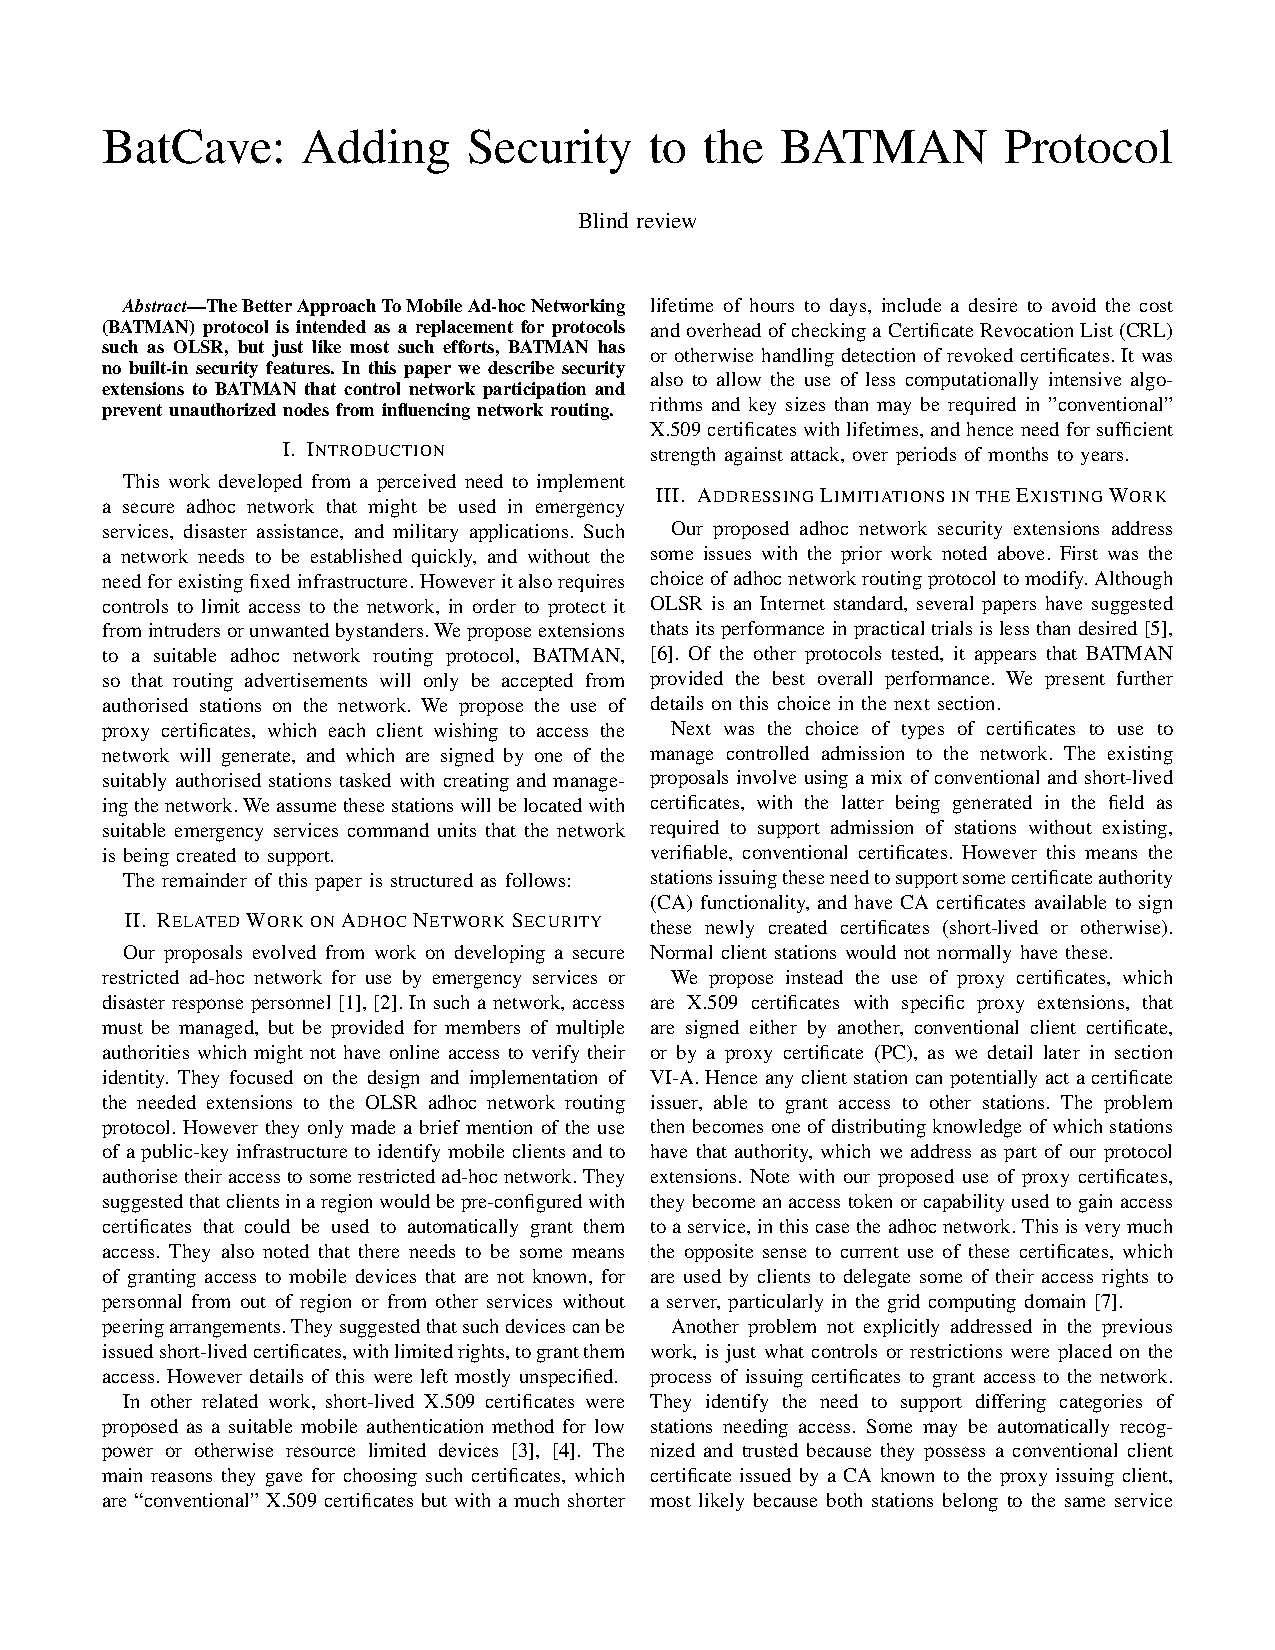
\includepdf[pages=-]{share/paper.pdf}

\end{document}